\documentclass{beamer}

\mode<presentation>
{
  \usetheme{default}      % or try Darmstadt, Madrid, Warsaw, ...
  \usecolortheme{default} % or try albatross, beaver, crane, ...
  \usefonttheme{default}  % or try serif, structurebold, ...
  \setbeamertemplate{navigation symbols}{}
  \setbeamertemplate{caption}[numbered]
} 

\usepackage[english]{babel}
\usepackage[utf8x]{inputenc}
\usepackage{tikz}
\usetikzlibrary{shapes,arrows}

\title{Formal Verification}
\subtitle{Securitate informatică}
\AtBeginSection[]{}

\setbeamertemplate{sidebar right}{}
\setbeamertemplate{footline}{%
\hfill\usebeamertemplate***{navigation symbols}
\hspace{1cm}\insertframenumber{}/\inserttotalframenumber}

\begin{document}

\begin{frame}
  \titlepage
  
\begin{flushright}
Mihai-Lica Pura\\
\end{flushright}

\end{frame}



\begin{frame}{Cuprins}

%Cursul va oferi o introducere în:

\begin{itemize}
\item
motivaţia verificării formale a protocoalelor de securitate;
\item
verificarea formală, pe scurt:
\begin{itemize}
\item
\textbf{modelarea} sistemelor funcţionale, paralele şi distribuite (cu accentul pe protocoale de securitate), 
\item
\textbf{specificarea} cerinţelor pentru aceste sisteme,
\item
\textbf{verificarea} dacă cerinţele sunt sau nu îndeplinite de către sisteme.
\end{itemize} 
\item
verificarea formală a protocoalelor de securitate.
\end{itemize} 
\end{frame}



\begin{frame}{Definiţie}

\begin{itemize}
\item
"… actul demonstrării sau infirmării corectitudinii algoritmilor care compun un sistem, având în vedere o anumită specificare formală sau proprietate, şi folosind metode matematice formale"\\

\item
"... limbaje, tehnici şi unelte matematice pentru specificarea şi verificarea sistemelor"\\

\item
"un set de unelte şi notaţii, cu o semantică formală, folosite pentru a specifica neambiguu cerinţele unui sistem, care admit demonstrarea de proprietăţi ale acelei specificări şi demonstrarea corectitudinii unei implementări în raport cu acea specificare"

\end{itemize}

\end{frame}



\begin{frame}{Exemplu - Prânzul filosofilor}

\begin{figure}
\includegraphics[scale=0.4]{images/filo}
\caption{\label{fig:filo}\url{http://ingenieroprendiz4ever.blogspot.ro/2012/06/la-cena-de-los-filosofos-aplicacion-de.html}}
\end{figure}
\end{frame}



\begin{frame}{Exemplu - Prânzul filosofilor}
\begin{itemize}
\item
Iniţial filosofii gândesc. Atunci când unui filosof i se face foame:
\item
filosoful ia furculiţa din stânga,
\item
filosoful ia furculiţa din dreapta şi apoi începe să mănânce.
\item
Când filosoful se satură, pune pe masă ambele furculiţe şi apoi o ia de la capăt.
\end{itemize}

\vspace{0.5cm}

Cum se poate modela acest sistem?
\end{frame}



\begin{frame}{Reţele Petri}
\begin{itemize}
\item
formalism elementar care permite modelarea sistemelor paralele şi distribuite
\item
propus de Adam Petri în 1962 în teza sa de doctorat "Kommunicaktion mit Automaten"
\item
descrie schimbările de stare ale unui sistem prin intermediul tranziţiilor
\end{itemize}

\vspace{0.5cm}

\begin{figure}
\includegraphics[scale=0.4]{images/pn_water}
\caption{\label{fig:pn_water}\url{https://fknussel.wordpress.com/2013/11/01/petri-nets-101/}}
\end{figure}

\end{frame}



\begin{frame}{Reţele Petri}
O reţea Petri conţine:

\begin{itemize}
\item
\textbf{places} - reprezintă stările şi/sau condiţiile care trebuie îndeplinite înainte ca o acţiune să poată avea loc
\item
\textbf{transitions} - reprezintă acţiuni
\item
places and transitions may be connected by \textbf{directed arcs}
\item
places may contain \textbf{tokens} that may move to other places by executing actions
\end{itemize}

\vspace{0.5cm}

\begin{figure}
\includegraphics[scale=0.4]{images/pn_bus}
\caption{\label{fig:pn_bus}\url{https://fknussel.wordpress.com/2013/11/01/petri-nets-101/}}
\end{figure}


\end{frame}



\begin{frame}{Reţele Petri}

Transition \textbf{One person gets on bus} may fire if there are tokens in place \textbf{Person waiting} and in place \textbf{Bus waiting}

\vspace{0.5cm}

Firing this transition once will remove a token from \textbf{Person waiting} and a token from \textbf{Bus waiting}, and will place a new token in \textbf{Person on bus} and a new token in \textbf{Bus waiting}

\vspace{0.5cm}

\begin{figure}
\includegraphics[scale=0.4]{images/pn_bus}
\caption{\label{fig:pn_bus}\url{https://fknussel.wordpress.com/2013/11/01/petri-nets-101/}}
\end{figure}
\end{frame}



\begin{frame}{Reţele Petri}
Modele interactive:

\vspace{0.5cm}

\url{http://www.informatik.uni-hamburg.de/TGI/PetriNets/introductions/aalst/}
\end{frame}



\begin{frame}{Exemplu - Prânzul filosofilor}
\begin{center}
\setlength{\unitlength}{.75ex}
\begin{picture}(64,44)(-2,-2)
%\put(-11,5){\makebox(4.5,3){\parbox[c][3\unitlength]{4.5\unitlength}{\large\sf Phil.~1}}}
%\put(-11,35){\makebox(4.5,3){\parbox[c][3\unitlength]{4.5\unitlength}{\large\sf Phil.~4}}}
%\put(63,5){\makebox(4.5,3){\parbox[c][3\unitlength]{4.5\unitlength}{\large\sf Phil.~2}}}
%\put(63,35){\makebox(4.5,3){\parbox[c][3\unitlength]{4.5\unitlength}{\large\sf Phil.~3}}}
%places
\multiput(0,0)(0,40){2}{\circle{4}}\multiput(60,0)(0,40){2}{\circle{4}}
\multiput(20,0)(10,0){3}{\circle{4}}\multiput(20,40)(10,0){3}{\circle{4}}
\multiput(10,10)(0,10){3}{\circle{4}}\multiput(50,10)(0,10){3}{\circle{4}}
%initial marking
\multiput(10,10)(0,10){2}{\circle*{1}}
\multiput(50,20)(0,10){2}{\circle*{1}}
\multiput(30,0)(10,0){2}{\circle*{1}}
\multiput(20,40)(10,0){2}{\circle*{1}}
\put(28.25,35.5){\makebox(4.5,3){\parbox[c][3\unitlength]{4.5\unitlength}{\small\sf fork}}}
\put(28.25,2){\makebox(4.5,3){\parbox[c][3\unitlength]{4.5\unitlength}{\small\sf fork}}}
\put(4,18.5){\makebox(4.5,3){\parbox[c][3\unitlength]{4.5\unitlength}{\small\sf fork}}}
\put(52.5,18.5){\makebox(4.5,3){\parbox[c][3\unitlength]{4.5\unitlength}{\small\sf fork}}}
% philosopher 1
\put(-2,8){\framebox(4,4){\(l_1\)}}
\put(8,10){\vector(-1,0){6}}\put(8.5,18.5){\vector(-1,-1){6.5}}
\put(0,8){\vector(0,-1){6}}
\put(8,-2){\framebox(4,4){\(r_1\)}}
\multiput(2,0)(10,0){2}{\vector(1,0){6}}
\put(20,-2){\oval(20,6)[b]}\put(10,-2){\vector(0,1){0}}
\put(18,8){\framebox(4,4){\(b_1\)}}
\put(20,2){\vector(0,1){6}}\put(18,10){\vector(-1,0){6}}
\put(22,8){\vector(1,-1){6.5}}\put(18,12){\vector(-1,1){6.5}}
\put(6.5,5){\makebox(4.5,3){\parbox[c][3\unitlength]{4.5\unitlength}{\small\sf thinking}}}
\put(17.5,-5){\makebox(4.5,3){\parbox[c][3\unitlength]{4.5\unitlength}{\small\sf eating}}}
% philosopher 2
\put(58,8){\framebox(4,4){\(r_2\)}}
\put(58,10){\vector(-1,0){6}}\put(51.5,18.5){\vector(1,-1){6.5}}
\put(60,2){\vector(0,1){6}}
\put(48,-2){\framebox(4,4){\(l_2\)}}
\multiput(42,0)(10,0){2}{\vector(1,0){6}}
\put(40,-2){\oval(20,6)[b]}\put(50,-2){\vector(0,1){0}}
\put(38,8){\framebox(4,4){\(b_2\)}}
\put(40,8){\vector(0,-1){6}}\put(48,10){\vector(-1,0){6}}
\put(38,8){\vector(-1,-1){6.5}}\put(42,12){\vector(1,1){6.5}}
\put(47.5,5){\makebox(4.5,3){\parbox[c][3\unitlength]{4.5\unitlength}{\small\sf eating}}}
\put(36.5,-5){\makebox(4.5,3){\parbox[c][3\unitlength]{4.5\unitlength}{\small\sf thinking}}}
% philosopher 3
\put(58,28){\framebox(4,4){\(l_3\)}}
\put(52,30){\vector(1,0){6}}\put(51.5,21.5){\vector(1,1){6.5}}
\put(60,32){\vector(0,1){6}}
\put(48,38){\framebox(4,4){\(r_3\)}}
\multiput(48,40)(10,0){2}{\vector(-1,0){6}}
\put(40,42){\oval(20,6)[t]}\put(50,42){\vector(0,-1){0}}
\put(38,28){\framebox(4,4){\(b_3\)}}
\put(40,38){\vector(0,-1){6}}\put(42,30){\vector(1,0){6}}
\put(38,32){\vector(-1,1){6.5}}\put(42,28){\vector(1,-1){6.5}}
\put(46.5,32){\makebox(4.5,3){\parbox[c][3\unitlength]{4.5\unitlength}{\small\sf thinking}}}
\put(37.5,42){\makebox(4.5,3){\parbox[c][3\unitlength]{4.5\unitlength}{\small\sf eating}}}
% philosopher 4
\put(-2,28){\framebox(4,4){\(r_4\)}}
\put(2,30){\vector(1,0){6}}\put(8.5,21.5){\vector(-1,1){6.5}}
\put(0,38){\vector(0,-1){6}}
\put(8,38){\framebox(4,4){\(l_4\)}}
\multiput(8,40)(10,0){2}{\vector(-1,0){6}}
\put(20,42){\oval(20,6)[t]}\put(10,42){\vector(0,-1){0}}
\put(18,28){\framebox(4,4){\(b_4\)}}
\put(20,32){\vector(0,1){6}}\put(12,30){\vector(1,0){6}}
\put(22,32){\vector(1,1){6.5}}\put(18,28){\vector(-1,-1){6.5}}
\put(7.5,32){\makebox(4.5,3){\parbox[c][3\unitlength]{4.5\unitlength}{\small\sf eating}}}
\put(16.5,42){\makebox(4.5,3){\parbox[c][3\unitlength]{4.5\unitlength}{\small\sf thinking}}}
\end{picture}
\end{center}
\begin{center}
Didier Buchs, cursul "Modélisation et vérification de logiciels" - Universitatea din Geneva
\end{center}
\end{frame}



\begin{frame}{Prânzul filosofilor - Proprietăţi}
\begin{itemize}
\item
Doi filosofi vecini pot mânca în acelaşi timp?
\item
Doi filosofi aflaţi faţă în faţă pot mânca în acelaşi timp?
\item
Se poate întâmpla ca filosofii să flămânzească până la moarte?
\item
Un anume filosof poate mânca în cele din urmă (presupunând că doreşte să facă acest lucru)?
\end{itemize}

\vspace{0.5cm}

Cum pot fi exprimate aceste întrebări ca şi proprietăţi ale reţelei Petri care modelează sistemul?
\end{frame}



\begin{frame}{Tipuri de reţele Petri}
\begin{itemize}
\item
only black tokens - \textbf{Place/Transition nets}

StrataGEM \url{https://github.com/mundacho/stratagem}
\item
colored tokens - \textbf{Colored Petri nets}

CPN Tools \url{http://cpntools.org/}
\item
tokens are terms of some Algebraic Abstract Data Types (AADT) - \textbf{Algebraic Petri nets}

AlPiNA \url{http://alpina.unige.ch/}
\end{itemize}

\vspace{0.5cm}

Există multe alte tipuri de reţele Petri şi instrumente asociate: \url{https://www.informatik.uni-hamburg.de/TGI/PetriNets/tools/quick.html}

\end{frame}



\begin{frame}{Algebraic Abstract Data Types - Exemplu booleans}
	Adt boolean
	
	Sorts \textbf{bool};
	
	Generators
	
\hspace{0.5cm}		\textbf{true} : bool;
		
\hspace{0.5cm}		\textbf{false} : bool;
		
%	Operations 
%		not : bool -> bool;
%		and : bool, bool -> bool;
%		or : bool, bool -> bool;
%		xor : bool, bool -> bool;
%		implies : bool, bool -> bool;
		
%	Axioms
%		not(true) = false;
%		not(false) = true;
		
%		and(true, $boolVar) = $boolVar;
%		and(false, $boolVar) = false;
		
%		or(true, $boolVar) = true;
%		or(false, $boolVar) = $boolVar;
		
%		xor(true, $boolVar) = not($boolVar);
%		xor(false, $boolVar) = $boolVar;
		
%		implies(false, $boolVar) = true;
%		implies(true, $boolVar) = $boolVar;

%	Variables
%		boolVar : bool;	
\end{frame}



\begin{frame}{Algebraic Abstract Data Types - Exemplu naturals}
	Adt naturals
	
	Sorts \textbf{nat};
	
	Generators
	
\hspace{0.5cm}		\textbf{zero} : nat;
		
\hspace{0.5cm}		\textbf{suc} : nat $\rightarrow$ nat;
		
	Operations
	
%		dec : nat -> nat;
\hspace{0.5cm}		\textbf{plus} : nat, nat $\rightarrow$ nat;
		
\hspace{0.5cm}		\textbf{minus} : nat, nat $\rightarrow$ nat;
		
%		times : nat, nat -> nat;
%		divide : nat, nat -> nat;
%		mod : nat, nat -> nat;
\hspace{0.5cm}		\textbf{gt} : nat, nat $\rightarrow$ bool;
		
%		lt : nat, nat -> bool;
%		ge : nat, nat -> bool;
%		le : nat, nat -> bool;
%		max : nat, nat -> nat;
%		min : nat, nat -> nat;
%		even : nat -> bool;

\end{frame}



\begin{frame}{Algebraic Abstract Data Types - Exemplu naturals (continuare)}
	Axioms
	
%		//dec
%		dec(suc($x)) = $x;

%		//plus
\hspace{0.5cm}		plus (zero, \$x) = \$x;

\hspace{0.5cm}		plus (suc(\$x), \$y) = suc (plus (\$x,\$y));

\vspace{0.25cm}

%		//minus
\hspace{0.5cm}		minus(\$x, zero) = \$x;

\hspace{0.5cm}		minus(suc(\$x), suc(\$y)) = minus(\$x, \$y);

\vspace{0.25cm}
		 
%		//times
%		times($x, zero) = zero;
%		times($x, suc($y)) = plus($x, times($x, $y));
		
%		//divide
%		if ge($x, $y) = true & gt($y, zero) = true then divide($x, $y) = suc(divide(minus($x, $y), $y));
%		if ge($x, $y) = false & gt($y, zero) = true then divide($x, $y) = zero;
		
%		//mod
%	    if gt($y, zero) = true then mod($x, $y) = minus($x, times($y, divide($x,$y)));

%		//gt
\hspace{0.5cm}		gt(zero, \$x) = false;

\hspace{0.5cm}		gt(suc(\$x),zero) = true;

\hspace{0.5cm}		gt(suc(\$y), suc(\$x)) = gt (\$y, \$x);

\vspace{0.25cm}
		
%		//st
%		lt(zero, suc(\$x)) = true;
%		lt(\$x, zero) = false;
%		lt(suc(\$y), suc(\$x)) = lt(\$y, \$x);
		
%		//ge
%		ge($x, $y) = not(lt($x,$y));
		
%		//se
%		le($x,$y) = not(gt($x, $y));
		
%		//max
%		if ge($x, $y) = true then max($x, $y) = $x;
%		if ge($x, $y) = false then max($x, $y) = $y;
		
%		//min
%		if le($x, $y) = true then max($x, $y) = $x;
%		if le($x, $y) = false then max($x, $y) = $y;
		
%		//even
%		even(zero) = true;
%		even(suc($x)) = not(even($x));
		
	Variables
	
\hspace{0.5cm}		x : nat;

\hspace{0.5cm}		y : nat;
%		n : nat;

\end{frame}



\begin{frame}{Algebraic Petri net - Exemplu - Sumator}
\begin{figure}
\includegraphics[scale=0.7]{images/sum}
\caption{\label{fig:sum}}
\end{figure}
\end{frame}



\begin{frame}{Prânzul filosofilor - APN}
\begin{figure}
\includegraphics[scale=0.5]{images/apn_filo}
\caption{\label{fig:apn_filo}\url{http://en.wikipedia.org/wiki/Algebraic_Petri_net}}
\end{figure}
\end{frame}



\begin{frame}{Prânzul filosofilor - AADT}
		Adt philosophers
		
		Sorts \textbf{philo};
		
		Generators
		
\hspace{0.5cm}			\textbf{p0} : philo;

\hspace{0.5cm}			\textbf{p}  : philo $\rightarrow$ philo;
			
		Operations
		
\hspace{0.5cm}			\textbf{leftFork} : philo $\rightarrow$ fork;
			
\hspace{0.5cm}			\textbf{rightFork} : philo $\rightarrow$ fork;
			
\hspace{0.5cm}			\textbf{philoOf} : fork $\rightarrow$ philo;
\end{frame}



\begin{frame}{Prânzul filosofilor - AADT (continuare)}
		Axioms
		
\hspace{0.5cm}			p(p(p0)) = p0;
			
\hspace{0.5cm}			leftFork(p0) = f0;
			
\hspace{0.5cm}			rightFork(p0) = f(f0);
			
\hspace{0.5cm}			philoOf(f0) = p0;
			
\hspace{0.5cm}			leftFork(p(\$vphilo)) = f(leftFork(\$vphilo));
			
\hspace{0.5cm}			rightFork(p(\$vphilo)) = f (rightFork(\$vphilo));
			
\hspace{0.5cm}			philoOf(f(\$vfork)) = p(philoOf(\$vfork));
			
		Variables
		
\hspace{0.5cm}			vphilo : philo;

\hspace{0.5cm}			vfork : fork;

\hspace{0.5cm}			vl : fork;

\hspace{0.5cm}			vr : fork;
\end{frame}



\begin{frame}{Prânzul filosofilor - AADT (continuare)}
		Adt fork
		
		Sorts \textbf{fork};
		
		Generators
		
\hspace{0.5cm}			\textbf{f0} : fork;
			
\hspace{0.5cm}			\textbf{f}  : fork $\rightarrow$ fork; 
			
		Axioms
		
\hspace{0.5cm}			f(f(f0)) = f0;
\end{frame}



\begin{frame}{Construirea spaţiului stărilor}
\begin{itemize}
\item
Starea unei reţele Petri este reprezentată de căre distribuţia jetoanelor în locuri
\item
Starea se schimbă de fiecare dată când se execută o tranziţie
\item
Spaţiul stărilor reprezintă mulţimea stărilor prin care trece o reţea Petri pornind din starea iniţală şi apoi executând toate tranziţiile posibile
\item
Poate fi reprezentat printr-un graf:
\begin{itemize}
\item
nodurile grafului corespund distribuţiei jetoanelor în locuri
\item
arcurile grafului corespund execuţiei tranziţiilor
\end{itemize}
\end{itemize}
\end{frame}



\begin{frame}{Spaţiul stărilor - Prânzul filosofilor}
\begin{center}

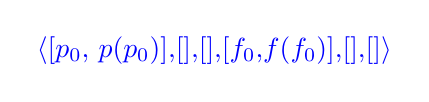
\begin{tikzpicture}
\node[blue] (p1) at (0,0) {$\langle$[$p_0$, $p(p_0)$],[],[],[$f_0$,$f(f_0)$],[],[]$\rangle$};
\end{tikzpicture}

\end{center}

\end{frame}



\begin{frame}{Spaţiul stărilor - Prânzul filosofilor}
\begin{center}

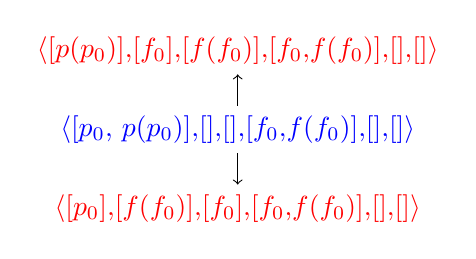
\begin{tikzpicture}
\node[blue] (p1) at (0,0) {$\langle$[$p_0$, $p(p_0)$],[],[],[$f_0$,$f(f_0)$],[],[]$\rangle$};

\node[red] (p2) at (0, 1) {$\langle$[$p(p_0)$],[$f_0$],[$f(f_0)$],[$f_0$,$f(f_0)$],[],[]$\rangle$};

\node[red] (p3) at (0, -1) {$\langle$[$p_0$],[$f(f_0)$],[$f_0$],[$f_0$,$f(f_0)$],[],[]$\rangle$};

\begin{scope}[every path/.style={->}]
       \draw (p1) -- (p2);
       \draw (p1) -- (p3); 
\end{scope} 

\end{tikzpicture}
\end{center}
\end{frame}



\begin{frame}{Spaţiul stărilor - Prânzul filosofilor}
\begin{center}

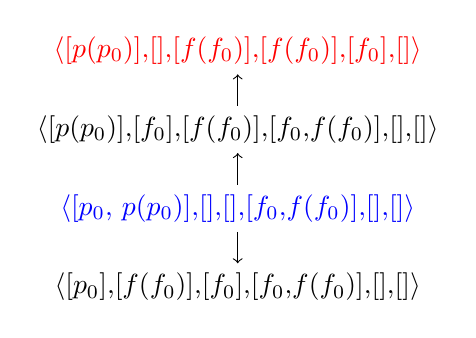
\begin{tikzpicture}
\node[blue] (p1) at (0,0) {$\langle$[$p_0$, $p(p_0)$],[],[],[$f_0$,$f(f_0)$],[],[]$\rangle$};

\node (p2) at (0, 1) {$\langle$[$p(p_0)$],[$f_0$],[$f(f_0)$],[$f_0$,$f(f_0)$],[],[]$\rangle$};

\node (p3) at (0, -1) {$\langle$[$p_0$],[$f(f_0)$],[$f_0$],[$f_0$,$f(f_0)$],[],[]$\rangle$};

\node[red] (p4) at (0, 2) {$\langle$[$p(p_0)$],[],[$f(f_0)$],[$f(f_0)$],[$f_0$],[]$\rangle$};

\begin{scope}[every path/.style={->}]
       \draw (p1) -- (p2);
       \draw (p1) -- (p3); 
       \draw (p2) -- (p4); 
\end{scope} 

\end{tikzpicture}

\end{center}
\end{frame}



\begin{frame}{Spaţiul stărilor - Prânzul filosofilor}
\begin{center}

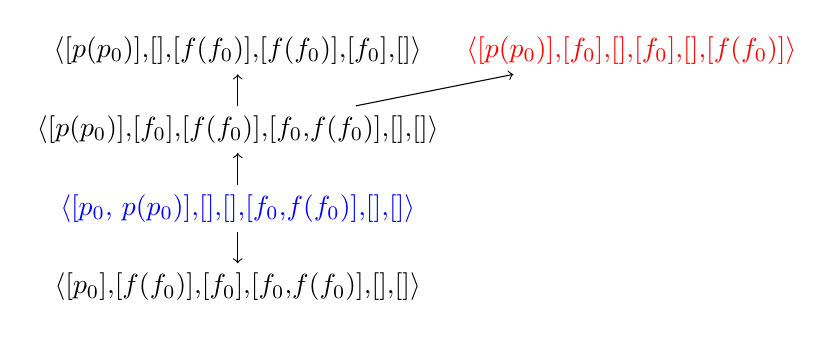
\begin{tikzpicture}
\node[blue] (p1) at (0,0) {$\langle$[$p_0$, $p(p_0)$],[],[],[$f_0$,$f(f_0)$],[],[]$\rangle$};

\node (p11) at (0, 1) {$\langle$[$p(p_0)$],[$f_0$],[$f(f_0)$],[$f_0$,$f(f_0)$],[],[]$\rangle$};

\node (p12) at (0, -1) {$\langle$[$p_0$],[$f(f_0)$],[$f_0$],[$f_0$,$f(f_0)$],[],[]$\rangle$};

\node (p111) at (0, 2) {$\langle$[$p(p_0)$],[],[$f(f_0)$],[$f(f_0)$],[$f_0$],[]$\rangle$};

\node[red] (p112) at (5, 2) {$\langle$[$p(p_0)$],[$f_0$],[],[$f_0$],[],[$f(f_0)$]$\rangle$};

\begin{scope}[every path/.style={->}]
       \draw (p1) -- (p11);
       \draw (p1) -- (p12); 
       \draw (p11) -- (p111); 
       \draw (p11) -- (p112); 
\end{scope} 

\end{tikzpicture}

\end{center}
\end{frame}



\begin{frame}{Spaţiul stărilor - Prânzul filosofilor}
\begin{center}

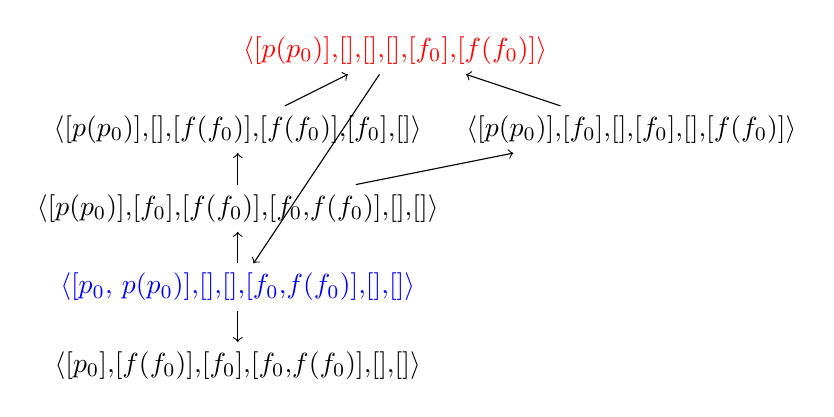
\begin{tikzpicture}
\node[blue] (p1) at (0,0) {$\langle$[$p_0$, $p(p_0)$],[],[],[$f_0$,$f(f_0)$],[],[]$\rangle$};

\node (p11) at (0, 1) {$\langle$[$p(p_0)$],[$f_0$],[$f(f_0)$],[$f_0$,$f(f_0)$],[],[]$\rangle$};

\node (p12) at (0, -1) {$\langle$[$p_0$],[$f(f_0)$],[$f_0$],[$f_0$,$f(f_0)$],[],[]$\rangle$};

\node (p111) at (0, 2) {$\langle$[$p(p_0)$],[],[$f(f_0)$],[$f(f_0)$],[$f_0$],[]$\rangle$};

\node (p112) at (5, 2) {$\langle$[$p(p_0)$],[$f_0$],[],[$f_0$],[],[$f(f_0)$]$\rangle$};

\node[red] (p11e) at (2, 3) {$\langle$[$p(p_0)$],[],[],[],[$f_0$],[$f(f_0)$]$\rangle$};

\begin{scope}[every path/.style={->}]
       \draw (p1) -- (p11);
       \draw (p1) -- (p12); 
       \draw (p11) -- (p111); 
       \draw (p11) -- (p112); 
       \draw (p111) -- (p11e); 
       \draw (p112) -- (p11e); 
       \draw (p11e) -- (p1); 
\end{scope} 

\end{tikzpicture}

\end{center}
\end{frame}



\begin{frame}{Spaţiul stărilor - Prânzul filosofilor}
\begin{center}

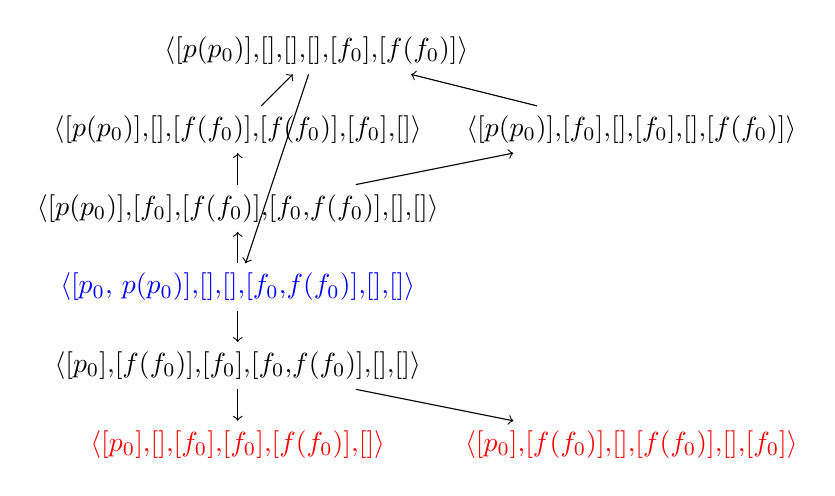
\begin{tikzpicture}
\node[blue] (p1) at (0,0) {$\langle$[$p_0$, $p(p_0)$],[],[],[$f_0$,$f(f_0)$],[],[]$\rangle$};

\node (p11) at (0, 1) {$\langle$[$p(p_0)$],[$f_0$],[$f(f_0)$],[$f_0$,$f(f_0)$],[],[]$\rangle$};

\node (p12) at (0, -1) {$\langle$[$p_0$],[$f(f_0)$],[$f_0$],[$f_0$,$f(f_0)$],[],[]$\rangle$};

\node (p111) at (0, 2) {$\langle$[$p(p_0)$],[],[$f(f_0)$],[$f(f_0)$],[$f_0$],[]$\rangle$};

\node (p112) at (5, 2) {$\langle$[$p(p_0)$],[$f_0$],[],[$f_0$],[],[$f(f_0)$]$\rangle$};

\node (p11e) at (1, 3) {$\langle$[$p(p_0)$],[],[],[],[$f_0$],[$f(f_0)$]$\rangle$};

\node[red] (p121) at (0, -2) {$\langle$[$p_0$],[],[$f_0$],[$f_0$],[$f(f_0)$],[]$\rangle$};

\node[red] (p122) at (5, -2) {$\langle$[$p_0$],[$f(f_0)$],[],[$f(f_0)$],[],[$f_0$]$\rangle$};

\begin{scope}[every path/.style={->}]
       \draw (p1) -- (p11);
       \draw (p1) -- (p12); 
       \draw (p11) -- (p111); 
       \draw (p11) -- (p112); 
       \draw (p111) -- (p11e); 
       \draw (p112) -- (p11e); 
       \draw (p11e) -- (p1); 
       \draw (p12) -- (p121); 
       \draw (p12) -- (p122); 
\end{scope} 

\end{tikzpicture}

\end{center}
\end{frame}



\begin{frame}{Spaţiul stărilor - Prânzul filosofilor}
\begin{center}

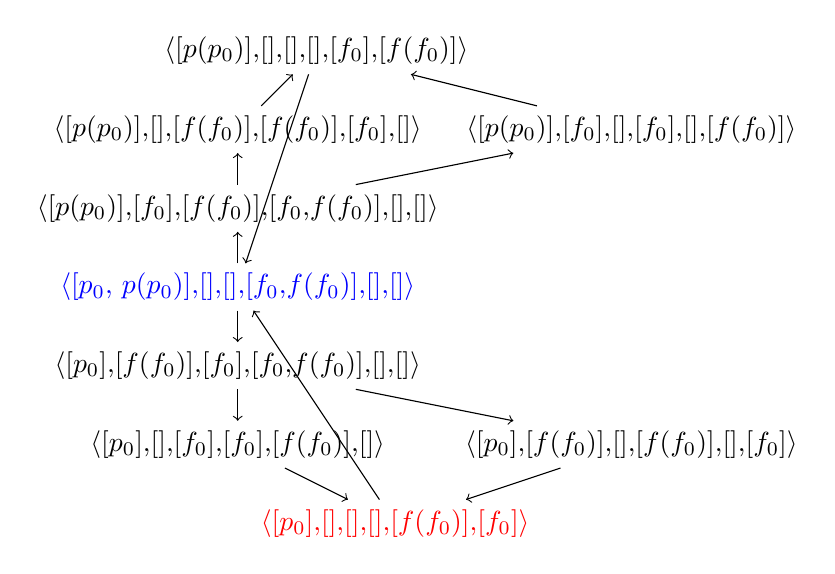
\begin{tikzpicture}
\node[blue] (p1) at (0,0) {$\langle$[$p_0$, $p(p_0)$],[],[],[$f_0$,$f(f_0)$],[],[]$\rangle$};

\node (p11) at (0, 1) {$\langle$[$p(p_0)$],[$f_0$],[$f(f_0)$],[$f_0$,$f(f_0)$],[],[]$\rangle$};

\node (p12) at (0, -1) {$\langle$[$p_0$],[$f(f_0)$],[$f_0$],[$f_0$,$f(f_0)$],[],[]$\rangle$};

\node (p111) at (0, 2) {$\langle$[$p(p_0)$],[],[$f(f_0)$],[$f(f_0)$],[$f_0$],[]$\rangle$};

\node (p112) at (5, 2) {$\langle$[$p(p_0)$],[$f_0$],[],[$f_0$],[],[$f(f_0)$]$\rangle$};

\node (p11e) at (1, 3) {$\langle$[$p(p_0)$],[],[],[],[$f_0$],[$f(f_0)$]$\rangle$};

\node (p121) at (0, -2) {$\langle$[$p_0$],[],[$f_0$],[$f_0$],[$f(f_0)$],[]$\rangle$};

\node (p122) at (5, -2) {$\langle$[$p_0$],[$f(f_0)$],[],[$f(f_0)$],[],[$f_0$]$\rangle$};

\node[red] (p12e) at (2, -3) {$\langle$[$p_0$],[],[],[],[$f(f_0)$],[$f_0$]$\rangle$};

\begin{scope}[every path/.style={->}]
       \draw (p1) -- (p11);
       \draw (p1) -- (p12); 
       \draw (p11) -- (p111); 
       \draw (p11) -- (p112); 
       \draw (p111) -- (p11e); 
       \draw (p112) -- (p11e); 
       \draw (p11e) -- (p1); 
       \draw (p12) -- (p121); 
       \draw (p12) -- (p122); 
       \draw (p121) -- (p12e);
       \draw (p122) -- (p12e);
       \draw (p12e) -- (p1);
\end{scope} 

\end{tikzpicture}

\end{center}
\end{frame}



\begin{frame}{Spaţiul stărilor - Prânzul filosofilor}
\begin{center}

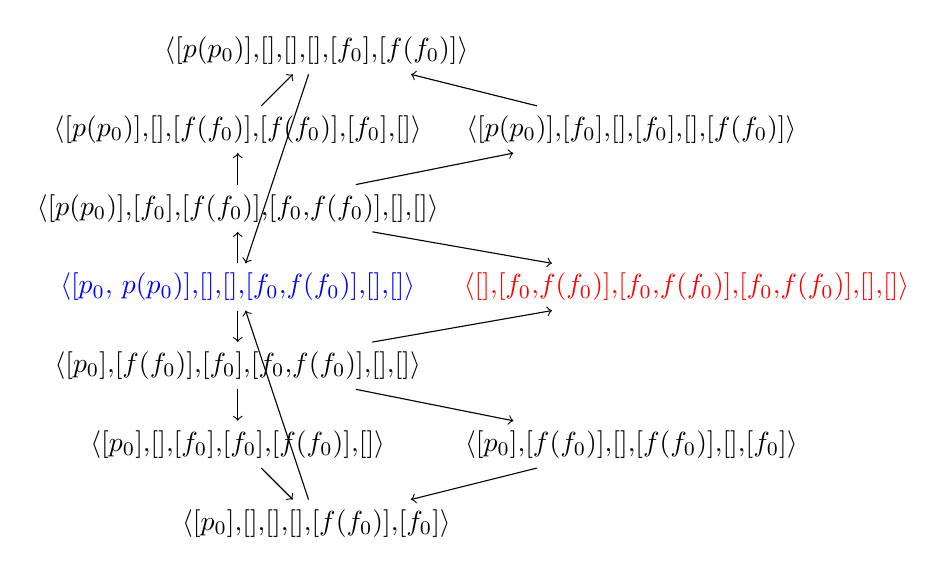
\begin{tikzpicture}
\node[blue] (p1) at (0,0) {$\langle$[$p_0$, $p(p_0)$],[],[],[$f_0$,$f(f_0)$],[],[]$\rangle$};

\node (p11) at (0, 1) {$\langle$[$p(p_0)$],[$f_0$],[$f(f_0)$],[$f_0$,$f(f_0)$],[],[]$\rangle$};

\node (p12) at (0, -1) {$\langle$[$p_0$],[$f(f_0)$],[$f_0$],[$f_0$,$f(f_0)$],[],[]$\rangle$};

\node (p111) at (0, 2) {$\langle$[$p(p_0)$],[],[$f(f_0)$],[$f(f_0)$],[$f_0$],[]$\rangle$};

\node (p112) at (5, 2) {$\langle$[$p(p_0)$],[$f_0$],[],[$f_0$],[],[$f(f_0)$]$\rangle$};

\node (p11e) at (1, 3) {$\langle$[$p(p_0)$],[],[],[],[$f_0$],[$f(f_0)$]$\rangle$};

\node (p121) at (0, -2) {$\langle$[$p_0$],[],[$f_0$],[$f_0$],[$f(f_0)$],[]$\rangle$};

\node (p122) at (5, -2) {$\langle$[$p_0$],[$f(f_0)$],[],[$f(f_0)$],[],[$f_0$]$\rangle$};

\node (p12e) at (1, -3) {$\langle$[$p_0$],[],[],[],[$f(f_0)$],[$f_0$]$\rangle$};

\node[red] (p2) at (5.7, 0) {$\langle$[],[$f_0$,$f(f_0)$],[$f_0$,$f(f_0)$],[$f_0$,$f(f_0)$],[],[]$\rangle$};

\begin{scope}[every path/.style={->}]
       \draw (p1) -- (p11);
       \draw (p1) -- (p12); 
       \draw (p11) -- (p111); 
       \draw (p11) -- (p112); 
       \draw (p111) -- (p11e); 
       \draw (p112) -- (p11e); 
       \draw (p11e) -- (p1); 
       \draw (p12) -- (p121); 
       \draw (p12) -- (p122); 
       \draw (p121) -- (p12e);
       \draw (p122) -- (p12e);
       \draw (p12e) -- (p1);
       \draw (p11) -- (p2);
       \draw (p12) -- (p2);
\end{scope} 

\end{tikzpicture}

\end{center}
\end{frame}



\begin{frame}{Spaţiul stărilor - Prânzul filosofilor}
\begin{center}

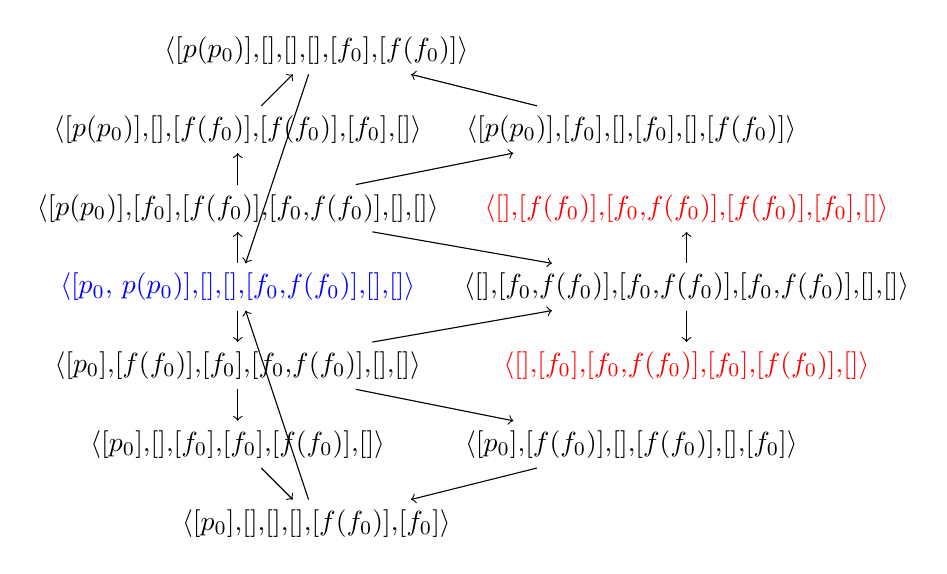
\begin{tikzpicture}
\node[blue] (p1) at (0,0) {$\langle$[$p_0$, $p(p_0)$],[],[],[$f_0$,$f(f_0)$],[],[]$\rangle$};

\node (p11) at (0, 1) {$\langle$[$p(p_0)$],[$f_0$],[$f(f_0)$],[$f_0$,$f(f_0)$],[],[]$\rangle$};

\node (p12) at (0, -1) {$\langle$[$p_0$],[$f(f_0)$],[$f_0$],[$f_0$,$f(f_0)$],[],[]$\rangle$};

\node (p111) at (0, 2) {$\langle$[$p(p_0)$],[],[$f(f_0)$],[$f(f_0)$],[$f_0$],[]$\rangle$};

\node (p112) at (5, 2) {$\langle$[$p(p_0)$],[$f_0$],[],[$f_0$],[],[$f(f_0)$]$\rangle$};

\node (p11e) at (1, 3) {$\langle$[$p(p_0)$],[],[],[],[$f_0$],[$f(f_0)$]$\rangle$};

\node (p121) at (0, -2) {$\langle$[$p_0$],[],[$f_0$],[$f_0$],[$f(f_0)$],[]$\rangle$};

\node (p122) at (5, -2) {$\langle$[$p_0$],[$f(f_0)$],[],[$f(f_0)$],[],[$f_0$]$\rangle$};

\node (p12e) at (1, -3) {$\langle$[$p_0$],[],[],[],[$f(f_0)$],[$f_0$]$\rangle$};

\node (p2) at (5.7, 0) {$\langle$[],[$f_0$,$f(f_0)$],[$f_0$,$f(f_0)$],[$f_0$,$f(f_0)$],[],[]$\rangle$};

\node[red] (p21) at (5.7, 1) {$\langle$[],[$f(f_0)$],[$f_0$,$f(f_0)$],[$f(f_0)$],[$f_0$],[]$\rangle$};

\node[red] (p22) at (5.7, -1) {$\langle$[],[$f_0$],[$f_0$,$f(f_0)$],[$f_0$],[$f(f_0)$],[]$\rangle$};

\begin{scope}[every path/.style={->}]
       \draw (p1) -- (p11);
       \draw (p1) -- (p12); 
       \draw (p11) -- (p111); 
       \draw (p11) -- (p112); 
       \draw (p111) -- (p11e); 
       \draw (p112) -- (p11e); 
       \draw (p11e) -- (p1); 
       \draw (p12) -- (p121); 
       \draw (p12) -- (p122); 
       \draw (p121) -- (p12e);
       \draw (p122) -- (p12e);
       \draw (p12e) -- (p1);
       \draw (p11) -- (p2);
       \draw (p12) -- (p2);
       \draw (p2) -- (p21);
		\draw (p2) -- (p22);       
\end{scope} 

\end{tikzpicture}

\end{center}
\end{frame}



\begin{frame}{Spaţiul stărilor - Prânzul filosofilor}
\begin{center}

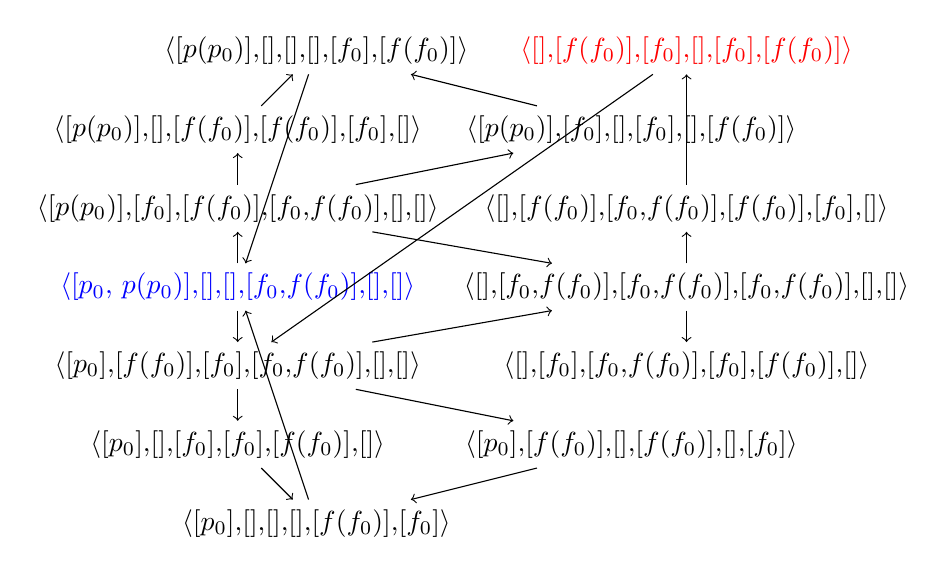
\begin{tikzpicture}
\node[blue] (p1) at (0,0) {$\langle$[$p_0$, $p(p_0)$],[],[],[$f_0$,$f(f_0)$],[],[]$\rangle$};

\node (p11) at (0, 1) {$\langle$[$p(p_0)$],[$f_0$],[$f(f_0)$],[$f_0$,$f(f_0)$],[],[]$\rangle$};

\node (p12) at (0, -1) {$\langle$[$p_0$],[$f(f_0)$],[$f_0$],[$f_0$,$f(f_0)$],[],[]$\rangle$};

\node (p111) at (0, 2) {$\langle$[$p(p_0)$],[],[$f(f_0)$],[$f(f_0)$],[$f_0$],[]$\rangle$};

\node (p112) at (5, 2) {$\langle$[$p(p_0)$],[$f_0$],[],[$f_0$],[],[$f(f_0)$]$\rangle$};

\node (p11e) at (1, 3) {$\langle$[$p(p_0)$],[],[],[],[$f_0$],[$f(f_0)$]$\rangle$};

\node (p121) at (0, -2) {$\langle$[$p_0$],[],[$f_0$],[$f_0$],[$f(f_0)$],[]$\rangle$};

\node (p122) at (5, -2) {$\langle$[$p_0$],[$f(f_0)$],[],[$f(f_0)$],[],[$f_0$]$\rangle$};

\node (p12e) at (1, -3) {$\langle$[$p_0$],[],[],[],[$f(f_0)$],[$f_0$]$\rangle$};

\node (p2) at (5.7, 0) {$\langle$[],[$f_0$,$f(f_0)$],[$f_0$,$f(f_0)$],[$f_0$,$f(f_0)$],[],[]$\rangle$};

\node (p21) at (5.7, 1) {$\langle$[],[$f(f_0)$],[$f_0$,$f(f_0)$],[$f(f_0)$],[$f_0$],[]$\rangle$};

\node (p22) at (5.7, -1) {$\langle$[],[$f_0$],[$f_0$,$f(f_0)$],[$f_0$],[$f(f_0)$],[]$\rangle$};

\node[red] (p211) at (5.7, 3) {$\langle$[],[$f(f_0)$],[$f_0$],[],[$f_0$],[$f(f_0)$]$\rangle$};

\begin{scope}[every path/.style={->}]
       \draw (p1) -- (p11);
       \draw (p1) -- (p12); 
       \draw (p11) -- (p111); 
       \draw (p11) -- (p112); 
       \draw (p111) -- (p11e); 
       \draw (p112) -- (p11e); 
       \draw (p11e) -- (p1); 
       \draw (p12) -- (p121); 
       \draw (p12) -- (p122); 
       \draw (p121) -- (p12e);
       \draw (p122) -- (p12e);
       \draw (p12e) -- (p1);
       \draw (p11) -- (p2);
       \draw (p12) -- (p2);
		\draw (p2) -- (p21);
		\draw (p2) -- (p22);       
		\draw (p21) -- (p211);              
       \draw (p211) -- (p12);
\end{scope} 

\end{tikzpicture}

\end{center}
\end{frame}



\begin{frame}{Spaţiul stărilor - Prânzul filosofilor}
\begin{center}

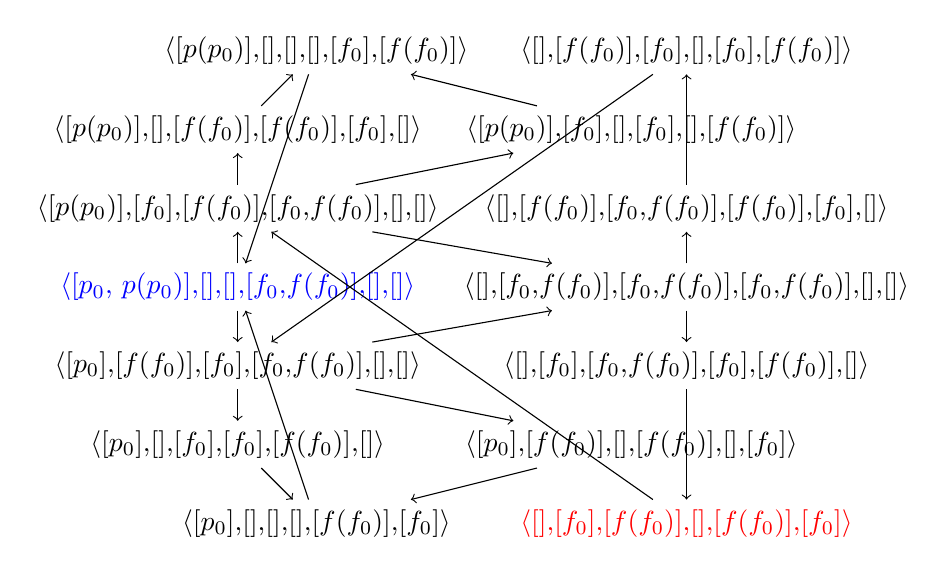
\begin{tikzpicture}
\node[blue] (p1) at (0,0) {$\langle$[$p_0$, $p(p_0)$],[],[],[$f_0$,$f(f_0)$],[],[]$\rangle$};

\node (p11) at (0, 1) {$\langle$[$p(p_0)$],[$f_0$],[$f(f_0)$],[$f_0$,$f(f_0)$],[],[]$\rangle$};

\node (p12) at (0, -1) {$\langle$[$p_0$],[$f(f_0)$],[$f_0$],[$f_0$,$f(f_0)$],[],[]$\rangle$};

\node (p111) at (0, 2) {$\langle$[$p(p_0)$],[],[$f(f_0)$],[$f(f_0)$],[$f_0$],[]$\rangle$};

\node (p112) at (5, 2) {$\langle$[$p(p_0)$],[$f_0$],[],[$f_0$],[],[$f(f_0)$]$\rangle$};

\node (p11e) at (1, 3) {$\langle$[$p(p_0)$],[],[],[],[$f_0$],[$f(f_0)$]$\rangle$};

\node (p121) at (0, -2) {$\langle$[$p_0$],[],[$f_0$],[$f_0$],[$f(f_0)$],[]$\rangle$};

\node (p122) at (5, -2) {$\langle$[$p_0$],[$f(f_0)$],[],[$f(f_0)$],[],[$f_0$]$\rangle$};

\node (p12e) at (1, -3) {$\langle$[$p_0$],[],[],[],[$f(f_0)$],[$f_0$]$\rangle$};

\node (p2) at (5.7, 0) {$\langle$[],[$f_0$,$f(f_0)$],[$f_0$,$f(f_0)$],[$f_0$,$f(f_0)$],[],[]$\rangle$};

\node (p21) at (5.7, 1) {$\langle$[],[$f(f_0)$],[$f_0$,$f(f_0)$],[$f(f_0)$],[$f_0$],[]$\rangle$};

\node (p22) at (5.7, -1) {$\langle$[],[$f_0$],[$f_0$,$f(f_0)$],[$f_0$],[$f(f_0)$],[]$\rangle$};

\node (p211) at (5.7, 3) {$\langle$[],[$f(f_0)$],[$f_0$],[],[$f_0$],[$f(f_0)$]$\rangle$};

\node[red] (p221) at (5.7, -3) {$\langle$[],[$f_0$],[$f(f_0)$],[],[$f(f_0)$],[$f_0$]$\rangle$};

\begin{scope}[every path/.style={->}]
       \draw (p1) -- (p11);
       \draw (p1) -- (p12); 
       \draw (p11) -- (p111); 
       \draw (p11) -- (p112); 
       \draw (p111) -- (p11e); 
       \draw (p112) -- (p11e); 
       \draw (p11e) -- (p1); 
       \draw (p12) -- (p121); 
       \draw (p12) -- (p122); 
       \draw (p121) -- (p12e);
       \draw (p122) -- (p12e);
       \draw (p12e) -- (p1);
       \draw (p11) -- (p2);
       \draw (p12) -- (p2);
		\draw (p2) -- (p21);
		\draw (p2) -- (p22);       
		\draw (p21) -- (p211);
		\draw (p22) -- (p221);
       \draw (p211) -- (p12);
       \draw (p221) -- (p11);
\end{scope} 

\end{tikzpicture}

\end{center}
\end{frame}



\begin{frame}{Spaţiul stărilor - Prânzul filosofilor}
\begin{center}

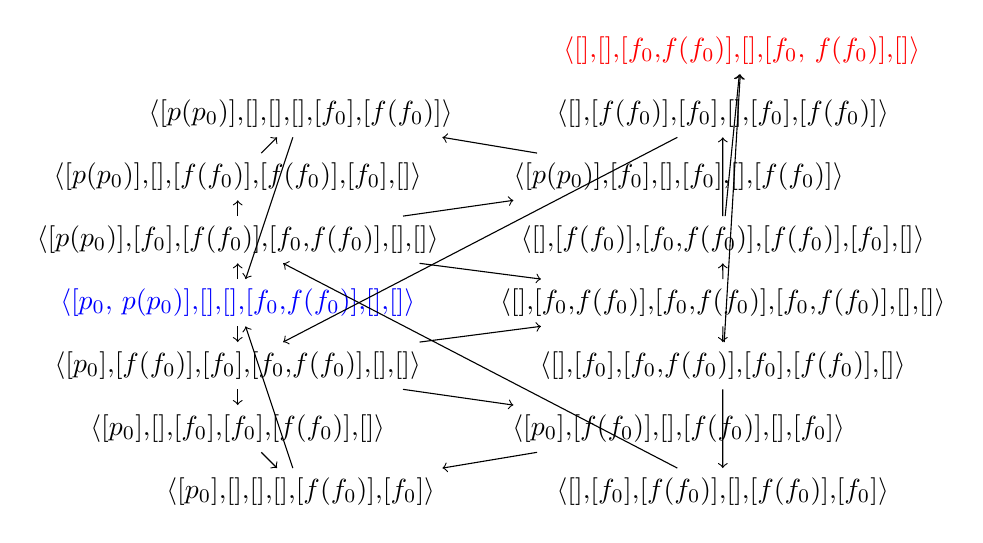
\begin{tikzpicture}[scale=0.8]
\node[blue] (p1) at (0,0) {$\langle$[$p_0$, $p(p_0)$],[],[],[$f_0$,$f(f_0)$],[],[]$\rangle$};

\node (p11) at (0, 1) {$\langle$[$p(p_0)$],[$f_0$],[$f(f_0)$],[$f_0$,$f(f_0)$],[],[]$\rangle$};

\node (p12) at (0, -1) {$\langle$[$p_0$],[$f(f_0)$],[$f_0$],[$f_0$,$f(f_0)$],[],[]$\rangle$};

\node (p111) at (0, 2) {$\langle$[$p(p_0)$],[],[$f(f_0)$],[$f(f_0)$],[$f_0$],[]$\rangle$};

\node (p112) at (7, 2) {$\langle$[$p(p_0)$],[$f_0$],[],[$f_0$],[],[$f(f_0)$]$\rangle$};

\node (p11e) at (1, 3) {$\langle$[$p(p_0)$],[],[],[],[$f_0$],[$f(f_0)$]$\rangle$};

\node (p121) at (0, -2) {$\langle$[$p_0$],[],[$f_0$],[$f_0$],[$f(f_0)$],[]$\rangle$};

\node (p122) at (7, -2) {$\langle$[$p_0$],[$f(f_0)$],[],[$f(f_0)$],[],[$f_0$]$\rangle$};

\node (p12e) at (1, -3) {$\langle$[$p_0$],[],[],[],[$f(f_0)$],[$f_0$]$\rangle$};

\node (p2) at (7.7, 0) {$\langle$[],[$f_0$,$f(f_0)$],[$f_0$,$f(f_0)$],[$f_0$,$f(f_0)$],[],[]$\rangle$};

\node (p21) at (7.7, 1) {$\langle$[],[$f(f_0)$],[$f_0$,$f(f_0)$],[$f(f_0)$],[$f_0$],[]$\rangle$};

\node (p22) at (7.7, -1) {$\langle$[],[$f_0$],[$f_0$,$f(f_0)$],[$f_0$],[$f(f_0)$],[]$\rangle$};

\node (p211) at (7.7, 3) {$\langle$[],[$f(f_0)$],[$f_0$],[],[$f_0$],[$f(f_0)$]$\rangle$};

\node (p221) at (7.7, -3) {$\langle$[],[$f_0$],[$f(f_0)$],[],[$f(f_0)$],[$f_0$]$\rangle$};

\node[red] (p2111) at (8, 4) {$\langle$[],[],[$f_0$,$f(f_0)$],[],[$f_0$, $f(f_0)$],[]$\rangle$};

\begin{scope}[every path/.style={->}]
       \draw (p1) -- (p11);
       \draw (p1) -- (p12); 
       \draw (p11) -- (p111); 
       \draw (p11) -- (p112); 
       \draw (p111) -- (p11e); 
       \draw (p112) -- (p11e); 
       \draw (p11e) -- (p1); 
       \draw (p12) -- (p121); 
       \draw (p12) -- (p122); 
       \draw (p121) -- (p12e);
       \draw (p122) -- (p12e);
       \draw (p12e) -- (p1);
       \draw (p11) -- (p2);
       \draw (p12) -- (p2);
		\draw (p2) -- (p21);
		\draw (p2) -- (p22);       
		\draw (p21) -- (p211);
		\draw (p22) -- (p221);
       \draw (p211) -- (p12);
       \draw (p221) -- (p11);
       \draw (p21) -- (p2111);
       \draw (p22) -- (p2111);
\end{scope} 

\end{tikzpicture}

\end{center}
\end{frame}



\begin{frame}{Spaţiul stărilor - Prânzul filosofilor}
\begin{center}

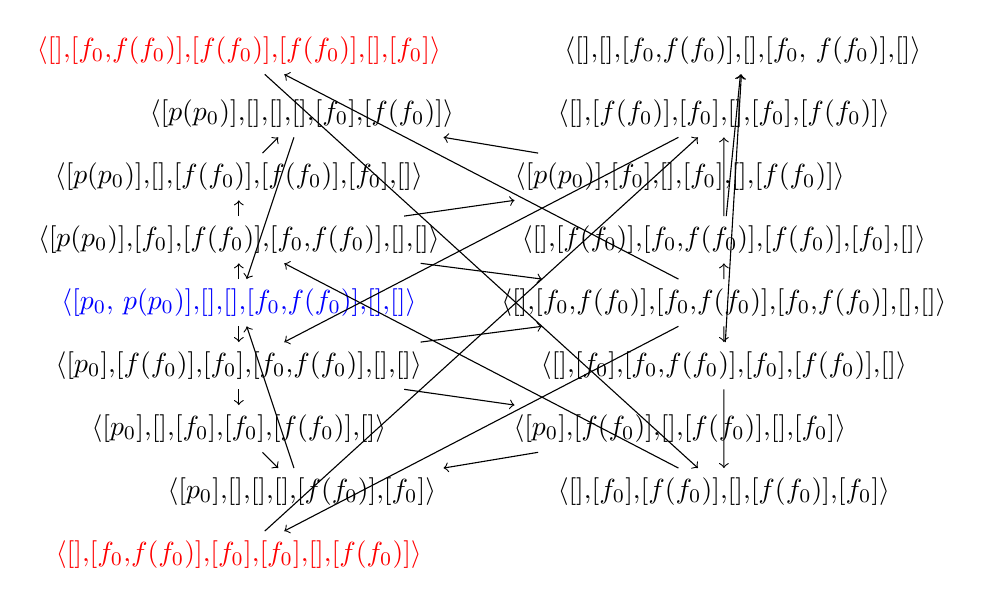
\begin{tikzpicture}[scale=0.8]
\node[blue] (p1) at (0,0) {$\langle$[$p_0$, $p(p_0)$],[],[],[$f_0$,$f(f_0)$],[],[]$\rangle$};

\node (p11) at (0, 1) {$\langle$[$p(p_0)$],[$f_0$],[$f(f_0)$],[$f_0$,$f(f_0)$],[],[]$\rangle$};

\node (p12) at (0, -1) {$\langle$[$p_0$],[$f(f_0)$],[$f_0$],[$f_0$,$f(f_0)$],[],[]$\rangle$};

\node (p111) at (0, 2) {$\langle$[$p(p_0)$],[],[$f(f_0)$],[$f(f_0)$],[$f_0$],[]$\rangle$};

\node (p112) at (7, 2) {$\langle$[$p(p_0)$],[$f_0$],[],[$f_0$],[],[$f(f_0)$]$\rangle$};

\node (p11e) at (1, 3) {$\langle$[$p(p_0)$],[],[],[],[$f_0$],[$f(f_0)$]$\rangle$};

\node (p121) at (0, -2) {$\langle$[$p_0$],[],[$f_0$],[$f_0$],[$f(f_0)$],[]$\rangle$};

\node (p122) at (7, -2) {$\langle$[$p_0$],[$f(f_0)$],[],[$f(f_0)$],[],[$f_0$]$\rangle$};

\node (p12e) at (1, -3) {$\langle$[$p_0$],[],[],[],[$f(f_0)$],[$f_0$]$\rangle$};

\node (p2) at (7.7, 0) {$\langle$[],[$f_0$,$f(f_0)$],[$f_0$,$f(f_0)$],[$f_0$,$f(f_0)$],[],[]$\rangle$};

\node (p21) at (7.7, 1) {$\langle$[],[$f(f_0)$],[$f_0$,$f(f_0)$],[$f(f_0)$],[$f_0$],[]$\rangle$};

\node (p22) at (7.7, -1) {$\langle$[],[$f_0$],[$f_0$,$f(f_0)$],[$f_0$],[$f(f_0)$],[]$\rangle$};

\node (p211) at (7.7, 3) {$\langle$[],[$f(f_0)$],[$f_0$],[],[$f_0$],[$f(f_0)$]$\rangle$};

\node (p221) at (7.7, -3) {$\langle$[],[$f_0$],[$f(f_0)$],[],[$f(f_0)$],[$f_0$]$\rangle$};

\node (p2111) at (8, 4) {$\langle$[],[],[$f_0$,$f(f_0)$],[],[$f_0$, $f(f_0)$],[]$\rangle$};

\node[red] (p23) at (0, 4) {$\langle$[],[$f_0$,$f(f_0)$],[$f(f_0)$],[$f(f_0)$],[],[$f_0$]$\rangle$};

\node[red] (p24) at (0, -4) {$\langle$[],[$f_0$,$f(f_0)$],[$f_0$],[$f_0$],[],[$f(f_0)$]$\rangle$};

\begin{scope}[every path/.style={->}]
       \draw (p1) -- (p11);
       \draw (p1) -- (p12); 
       \draw (p11) -- (p111); 
       \draw (p11) -- (p112); 
       \draw (p111) -- (p11e); 
       \draw (p112) -- (p11e); 
       \draw (p11e) -- (p1); 
       \draw (p12) -- (p121); 
       \draw (p12) -- (p122); 
       \draw (p121) -- (p12e);
       \draw (p122) -- (p12e);
       \draw (p12e) -- (p1);
       \draw (p11) -- (p2);
       \draw (p12) -- (p2);
		\draw (p2) -- (p21);
		\draw (p2) -- (p22);       
		\draw (p21) -- (p211);
		\draw (p22) -- (p221);
       \draw (p211) -- (p12);
       \draw (p221) -- (p11);
       \draw (p21) -- (p2111);
       \draw (p22) -- (p2111);
   		\draw (p2) -- (p23);
		\draw (p2) -- (p24);       
		\draw (p23) -- (p221);       
		\draw (p24) -- (p211);       
\end{scope} 

\end{tikzpicture}

\end{center}
\end{frame}



\begin{frame}{Spaţiul stărilor - Prânzul filosofilor}
\begin{center}

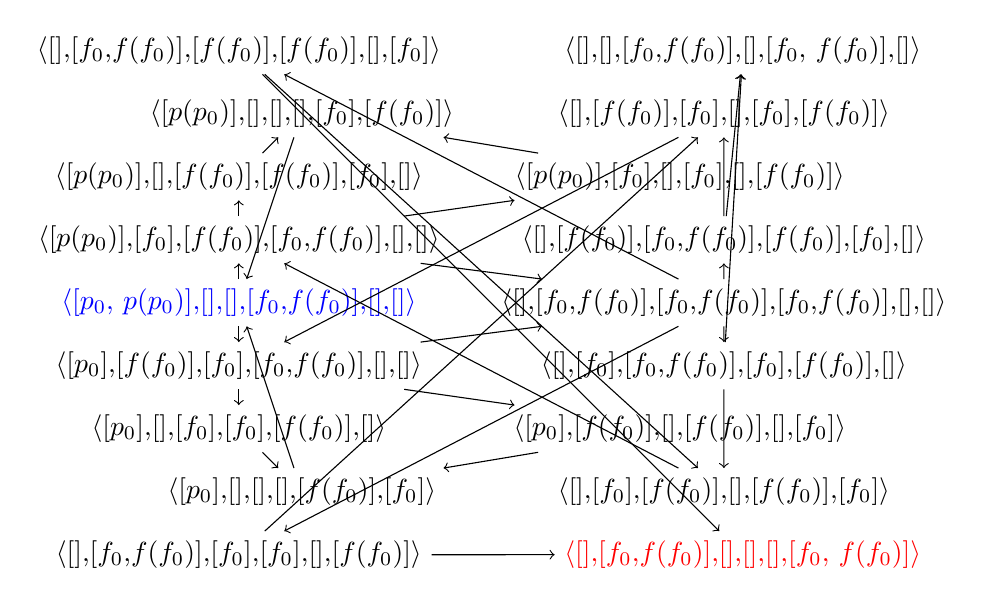
\begin{tikzpicture}[scale=0.8]
\node[blue] (p1) at (0,0) {$\langle$[$p_0$, $p(p_0)$],[],[],[$f_0$,$f(f_0)$],[],[]$\rangle$};

\node (p11) at (0, 1) {$\langle$[$p(p_0)$],[$f_0$],[$f(f_0)$],[$f_0$,$f(f_0)$],[],[]$\rangle$};

\node (p12) at (0, -1) {$\langle$[$p_0$],[$f(f_0)$],[$f_0$],[$f_0$,$f(f_0)$],[],[]$\rangle$};

\node (p111) at (0, 2) {$\langle$[$p(p_0)$],[],[$f(f_0)$],[$f(f_0)$],[$f_0$],[]$\rangle$};

\node (p112) at (7, 2) {$\langle$[$p(p_0)$],[$f_0$],[],[$f_0$],[],[$f(f_0)$]$\rangle$};

\node (p11e) at (1, 3) {$\langle$[$p(p_0)$],[],[],[],[$f_0$],[$f(f_0)$]$\rangle$};

\node (p121) at (0, -2) {$\langle$[$p_0$],[],[$f_0$],[$f_0$],[$f(f_0)$],[]$\rangle$};

\node (p122) at (7, -2) {$\langle$[$p_0$],[$f(f_0)$],[],[$f(f_0)$],[],[$f_0$]$\rangle$};

\node (p12e) at (1, -3) {$\langle$[$p_0$],[],[],[],[$f(f_0)$],[$f_0$]$\rangle$};

\node (p2) at (7.7, 0) {$\langle$[],[$f_0$,$f(f_0)$],[$f_0$,$f(f_0)$],[$f_0$,$f(f_0)$],[],[]$\rangle$};

\node (p21) at (7.7, 1) {$\langle$[],[$f(f_0)$],[$f_0$,$f(f_0)$],[$f(f_0)$],[$f_0$],[]$\rangle$};

\node (p22) at (7.7, -1) {$\langle$[],[$f_0$],[$f_0$,$f(f_0)$],[$f_0$],[$f(f_0)$],[]$\rangle$};

\node (p211) at (7.7, 3) {$\langle$[],[$f(f_0)$],[$f_0$],[],[$f_0$],[$f(f_0)$]$\rangle$};

\node (p221) at (7.7, -3) {$\langle$[],[$f_0$],[$f(f_0)$],[],[$f(f_0)$],[$f_0$]$\rangle$};

\node (p2111) at (8, 4) {$\langle$[],[],[$f_0$,$f(f_0)$],[],[$f_0$, $f(f_0)$],[]$\rangle$};

\node (p23) at (0, 4) {$\langle$[],[$f_0$,$f(f_0)$],[$f(f_0)$],[$f(f_0)$],[],[$f_0$]$\rangle$};

\node (p24) at (0, -4) {$\langle$[],[$f_0$,$f(f_0)$],[$f_0$],[$f_0$],[],[$f(f_0)$]$\rangle$};

\node[red] (p2112) at (8, -4) {$\langle$[],[$f_0$,$f(f_0)$],[],[],[],[$f_0$, $f(f_0)$]$\rangle$};

\begin{scope}[every path/.style={->}]
       \draw (p1) -- (p11);
       \draw (p1) -- (p12); 
       \draw (p11) -- (p111); 
       \draw (p11) -- (p112); 
       \draw (p111) -- (p11e); 
       \draw (p112) -- (p11e); 
       \draw (p11e) -- (p1); 
       \draw (p12) -- (p121); 
       \draw (p12) -- (p122); 
       \draw (p121) -- (p12e);
       \draw (p122) -- (p12e);
       \draw (p12e) -- (p1);
       \draw (p11) -- (p2);
       \draw (p12) -- (p2);
		\draw (p2) -- (p21);
		\draw (p2) -- (p22);       
		\draw (p21) -- (p211);
		\draw (p22) -- (p221);
       \draw (p211) -- (p12);
       \draw (p221) -- (p11);
       \draw (p21) -- (p2111);
       \draw (p22) -- (p2111);
   		\draw (p2) -- (p23);
		\draw (p2) -- (p24);       
		\draw (p23) -- (p221);       
		\draw (p24) -- (p211);       
		\draw (p23) -- (p2112);       
		\draw (p24) -- (p2112);       
\end{scope} 

\end{tikzpicture}

\end{center}
\end{frame}



\begin{frame}{Spaţiul stărilor - Prânzul filosofilor - 2 filosofi - 18 stări}
\begin{center}

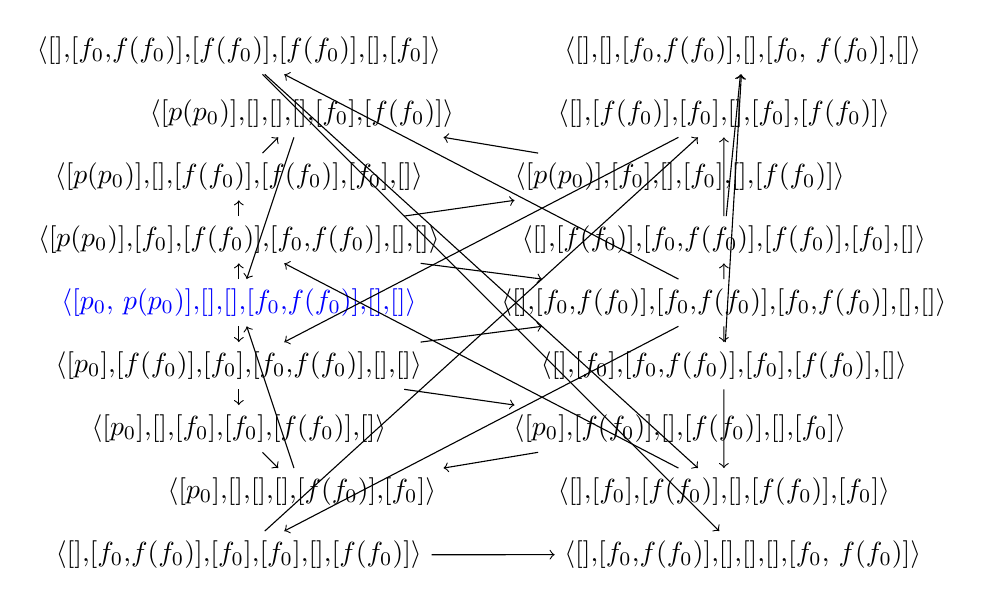
\begin{tikzpicture}[scale=0.8]
\node[blue] (p1) at (0,0) {$\langle$[$p_0$, $p(p_0)$],[],[],[$f_0$,$f(f_0)$],[],[]$\rangle$};

\node (p11) at (0, 1) {$\langle$[$p(p_0)$],[$f_0$],[$f(f_0)$],[$f_0$,$f(f_0)$],[],[]$\rangle$};

\node (p12) at (0, -1) {$\langle$[$p_0$],[$f(f_0)$],[$f_0$],[$f_0$,$f(f_0)$],[],[]$\rangle$};

\node (p111) at (0, 2) {$\langle$[$p(p_0)$],[],[$f(f_0)$],[$f(f_0)$],[$f_0$],[]$\rangle$};

\node (p112) at (7, 2) {$\langle$[$p(p_0)$],[$f_0$],[],[$f_0$],[],[$f(f_0)$]$\rangle$};

\node (p11e) at (1, 3) {$\langle$[$p(p_0)$],[],[],[],[$f_0$],[$f(f_0)$]$\rangle$};

\node (p121) at (0, -2) {$\langle$[$p_0$],[],[$f_0$],[$f_0$],[$f(f_0)$],[]$\rangle$};

\node (p122) at (7, -2) {$\langle$[$p_0$],[$f(f_0)$],[],[$f(f_0)$],[],[$f_0$]$\rangle$};

\node (p12e) at (1, -3) {$\langle$[$p_0$],[],[],[],[$f(f_0)$],[$f_0$]$\rangle$};

\node (p2) at (7.7, 0) {$\langle$[],[$f_0$,$f(f_0)$],[$f_0$,$f(f_0)$],[$f_0$,$f(f_0)$],[],[]$\rangle$};

\node (p21) at (7.7, 1) {$\langle$[],[$f(f_0)$],[$f_0$,$f(f_0)$],[$f(f_0)$],[$f_0$],[]$\rangle$};

\node (p22) at (7.7, -1) {$\langle$[],[$f_0$],[$f_0$,$f(f_0)$],[$f_0$],[$f(f_0)$],[]$\rangle$};

\node (p211) at (7.7, 3) {$\langle$[],[$f(f_0)$],[$f_0$],[],[$f_0$],[$f(f_0)$]$\rangle$};

\node (p221) at (7.7, -3) {$\langle$[],[$f_0$],[$f(f_0)$],[],[$f(f_0)$],[$f_0$]$\rangle$};

\node (p2111) at (8, 4) {$\langle$[],[],[$f_0$,$f(f_0)$],[],[$f_0$, $f(f_0)$],[]$\rangle$};

\node (p23) at (0, 4) {$\langle$[],[$f_0$,$f(f_0)$],[$f(f_0)$],[$f(f_0)$],[],[$f_0$]$\rangle$};

\node (p24) at (0, -4) {$\langle$[],[$f_0$,$f(f_0)$],[$f_0$],[$f_0$],[],[$f(f_0)$]$\rangle$};

\node (p2112) at (8, -4) {$\langle$[],[$f_0$,$f(f_0)$],[],[],[],[$f_0$, $f(f_0)$]$\rangle$};

\begin{scope}[every path/.style={->}]
       \draw (p1) -- (p11);
       \draw (p1) -- (p12); 
       \draw (p11) -- (p111); 
       \draw (p11) -- (p112); 
       \draw (p111) -- (p11e); 
       \draw (p112) -- (p11e); 
       \draw (p11e) -- (p1); 
       \draw (p12) -- (p121); 
       \draw (p12) -- (p122); 
       \draw (p121) -- (p12e);
       \draw (p122) -- (p12e);
       \draw (p12e) -- (p1);
       \draw (p11) -- (p2);
       \draw (p12) -- (p2);
		\draw (p2) -- (p21);
		\draw (p2) -- (p22);       
		\draw (p21) -- (p211);
		\draw (p22) -- (p221);
       \draw (p211) -- (p12);
       \draw (p221) -- (p11);
       \draw (p21) -- (p2111);
       \draw (p22) -- (p2111);
   		\draw (p2) -- (p23);
		\draw (p2) -- (p24);       
		\draw (p23) -- (p221);       
		\draw (p24) -- (p211);       
		\draw (p23) -- (p2112);       
		\draw (p24) -- (p2112);       
\end{scope} 

\end{tikzpicture}

\end{center}
\end{frame}



\begin{frame}{Modelarea versus proiectarea sistemelor}

\textbf{Modelarea sistemelor}: Ce sistem să se producă?

\vspace{0.5cm}

versus

\vspace{0.5cm}

\textbf{Proiectarea şi implementarea sistemelor}: Cum se produce sistemul respectiv?

\vspace{0.5cm}

Modelarea foloseşte limbaje expresive pentru a descrie funcţionalităţile dorite ale sistemului în cauză.

\end{frame}



\begin{frame}{Validarea versus Verificarea sistemelor}

\textbf{Validarea sistemelor}: Producem produsul corect?

\vspace{0.5cm}

versus

\vspace{0.5cm}

\textbf{Verificarea sistemelor}: Producem corect produsul?

\vspace{0.5cm}

Verificarea sistemelor controlează dacă sistemul îndeplineşte corect funcţionalităţile specificate.
\end{frame}



\begin{frame}{Analiza versus Modelarea sistemelor}

\textbf{Analiza}
\begin{itemize}
\item
reprezintă domeniile problemă din mai multe perspective
\item
descoperă caracteristcile sistemului
\end{itemize}

\textbf{Modelarea sistemelor}
\begin{itemize}
\item
sistemul este descris în întregime şi neambiguu
\item
foloseşte un limbaj foarte expresiv, adaptat domeniului problemelor avute în vedere
\item
se concentreaza pe aspecte funcţionale sau non-funcţionale
\end{itemize}

\end{frame}



\begin{frame}{Specificarea formală}
"Exprimarea într-un limbaj formal şi la un anumit nivel de abstractizare, a unei colecţii de proprietăţi pe care un sistem ar trebui să le îndeplinească".

\end{frame}



\begin{frame}{Specificarea formală}
Caracteristicile unei specificări formale:

\begin{itemize}
\item
\textbf{Adecvată} - să descrie într-un mod potrivit problema la care se referă
\item
\textbf{Consistentă} - interpretarea sa din punct de vedere semantic să fie plină de înţeles
\item
\textbf{Nu trebuie să fie ambiguă} - nu trebuie să aibă mai multe interpretări, toate adevărate
\item
\textbf{Minimală} - să se refere numai la proprietăţile relevante ale problemei
\end{itemize}
\end{frame}



\begin{frame}{Specificarea formală}
\begin{itemize}
\item
Rezultatele verificării formale depind de calitatea specificărilor formale: \textbf{modelul verificat va fi la fel de bun ca şi specificarea formală care stă la baza sa}
\item
Orice greşeală sau inadvertenţă de la acest nivel se va propaga şi asupra verificării formale propriu-zise.
\item
Specificarea formală ca şi modelul de verificat trebuie deci ele însele validate.
\end{itemize}
\end{frame}



\begin{frame}{Specificarea formală: proprietăţi ale sistemelor}
\begin{itemize}
\item
\textbf{Safety}: sistemul nu ajunge niciodată într-o stare nepotrivită 

- o anumită proprietate este valabilă de-a lungul întregii execuţii

ex: deadlock freedom, mutual exclusion

\item
\textbf{Liveness}: sistemul progresează în sarcina pe care o îndeplineşte

- unele acţiuni au loc infinit de des

\item
\textbf{Inevitability}: în cele din urmă, un anumit lucru va avea loc
\item
\textbf{Response}: ori de câte ori are loc X, în cele din urmă va avea loc şi Y

ex: sistemul răspunde la fiecare mesaj primit, fiecare cerere este rezolvată la un moment dat

\item
\textbf{Fairness assumptions}: X are loc, presupunând că procesorul este partajat de către toate procesele
\end{itemize}
\end{frame}



\begin{frame}{De ce să se utilizeze metodele formale?}
În prezent calculatoarele au devenit o prezenţă ubicuuă: calculatoare presonale, telefoane inteligente, tablete, ceasuri, maşini, trenuri, avioane, ş.a.

\vspace{0.5cm}

Sistemele software devin din ce în ce mai complexe.

\begin{itemize}
\item
producerea de software lipsit de bug-uri este din ce în ce mai dificilă
\item
efectele negative ale bug-urilor pot fi enorme: financiar, reputaţie, vieţi omeneşti
\item
cu cât o eroare este descoperită mai târziu, cu atât costul eliminării ei este mai mare
\end{itemize}
\end{frame}



\begin{frame}{(In)famous bugs}

European Space Agency's Ariane 5 Flight 501 (US\$1 billion) - destroyed 40 seconds after takeoff (June 4, 1996) - self-destructed due to a \textbf{bug in the on-board guidance software}

\vspace{0.5cm}

Smart ship USS Yorktown - dead in the water for nearly 3 hours - \textbf{divide by zero} error (1997)

\vspace{0.5cm}

OpenSSL vulnerability (introduced 2012, disclosed April 2014) - \textbf{removed confidentiality} from affected services

\begin{itemize}
\item
\url{http://www.computerworld.com/article/2515483/enterprise-applications/epic-failures--11-infamous-software-bugs.html}
\item
\url{https://en.wikipedia.org/wiki/List_of_software_bugs}
\end{itemize}

\end{frame}



\begin{frame}{(In)famous bugs}
Debugging Day - September 9

\vspace{0.5cm}

\begin{itemize}
\item
Descoperire bug-uri după ce sistemul este deja distribuit la clienţi (în urma efectelor produse)
\item
Corectare bug-uri în codul sursă
\item
Redistribuire sistem sau distribuire patch-uri
\end{itemize}

versus

\begin{itemize}
\item
descoperire erori de proiectare în modelul sistemului (verificare formală)
\item
implementare corectă distribuită la clienţi
\end{itemize}
\end{frame}



\begin{frame}{Aplicabilitatea metodelor formale}
Nu pot fi aplicate pentru a analiza automat toate proprietăţile tuturor programelor scrise

\begin{itemize}
\item
programele sunt în general mult \textbf{prea mari}
\item
problemele respective ar putea fi \textbf{indecidabile} în principiu

The \textbf{halting problem} is undecidable: there is no computer program that can correctly determine, given any program P as input, whether P eventually halts when run with a particular given input. (\url{https://en.wikipedia.org/wiki/Halting_problem})
\end{itemize}

Metodele formale se folosesc pentru:

\begin{itemize}
\item
părţile \textbf{critice} ale sistemelor
\item
subclase decidabile de probleme sau proprietăţi
\end{itemize}

\end{frame}



\begin{frame}{Aplicabilitatea metodelor formale}
Comunicaţii
\begin{itemize}
\item
verificarea şi testarea protocoalelor de comunicaţii (inclusiv proprietăţi de securitate)
\item
evaluarea performanţelor (throughput, queuing time, energy consumption, etc.)
\end{itemize}

Sisteme critice din punct de vedere al siguranţei
\begin{itemize}
\item
sistemele de comandă şi control ale aeronavelor
\item
sistemele de control ale traficului aerian
\item
sistemele de comandă ale traficului feroviar
\end{itemize}

Proiectarea componentelor hardware
\begin{itemize}
\item
procesoare, memorii cahe, interfeţe periferice, magistrale
\end{itemize}
\end{frame}



\begin{frame}{Metode de verificare formală}
\begin{itemize}
\item
Verificarea modelelor - \textbf{Model checking}
(verificatoare de modele)

- Exemplificată în slide-urile anterioare
\item
Demonstrarea teoremelor - \textbf{Theorem proving}
(demonstratoare de teoreme)
\item
Verificarea echivalenţei - \textbf{Equivalence checking}
(verificatoare de echivalenţă)
\end{itemize}
\end{frame}



\begin{frame}{Verificarea modelelor}
Construirea şi explorarea sistematică exhaustivă a spaţiului stărilor modelului matematic al sistemului

\vspace{0.5cm}

\begin{enumerate}
\item
Construirea unui model al sistemului de verificat
- limbaj de descriere a sistemului

ex: reţele Petri algebrice pentru prânzul filosofilor
\item
Specificarea proprietăţilor sistemului care trebuie verificate
- limbaj de descriere a proprietăţilor

\item
Verificarea propriu-zisă
\end{enumerate}
\end{frame}



\begin{frame}{Verificarea modelelor}
Instrumente special create
\begin{itemize}
\item
Intrare: 
\begin{itemize}
\item
modelul sistemului
\item
proprietăţile care trebuie verificate
\end{itemize}
\item
Ieşire
\begin{itemize}
\item
modelul are proprietatea/proprietăţile specificate
\item
modelul NU are proprietatea/proprietăţile specificate
\begin{itemize}
\item
\textbf{contraexemplu} - configuraţie a sistemului în care proprietate nu este îndeplinită
\end{itemize}
\end{itemize}
\end{itemize}
\end{frame}



\begin{frame}{Verificarea modelelor - AlPiNA - Prânzul filosofilor}
\begin{figure}
\centering
\includegraphics[scale=0.32]{images/alpina1}
\end{figure}
\end{frame}



\begin{frame}{Verificarea modelelor - AlPiNA - Prânzul filosofilor}
\begin{figure}
\centering
\includegraphics[scale=0.32]{images/alpina2}
\end{figure}
\end{frame}



\begin{frame}{Verificarea modelelor - AlPiNA - Prânzul filosofilor}
\begin{figure}
\centering
\includegraphics[scale=0.32]{images/alpina3}
\end{figure}
\end{frame}



\begin{frame}{Verificarea modelelor - AlPiNA - Prânzul filosofilor}
\begin{center}

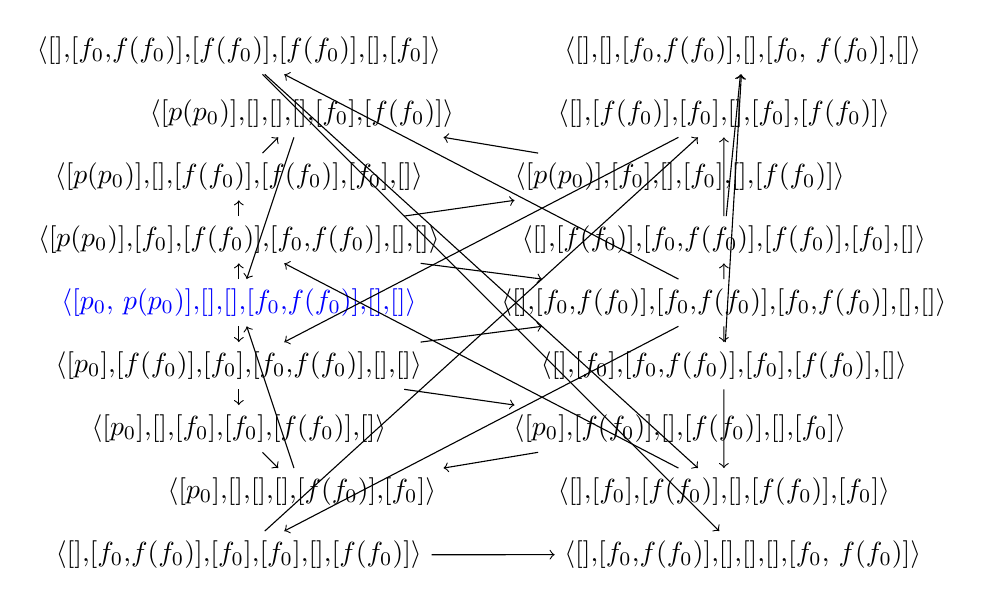
\begin{tikzpicture}[scale=0.8]
\node[blue] (p1) at (0,0) {$\langle$[$p_0$, $p(p_0)$],[],[],[$f_0$,$f(f_0)$],[],[]$\rangle$};

\node (p11) at (0, 1) {$\langle$[$p(p_0)$],[$f_0$],[$f(f_0)$],[$f_0$,$f(f_0)$],[],[]$\rangle$};

\node (p12) at (0, -1) {$\langle$[$p_0$],[$f(f_0)$],[$f_0$],[$f_0$,$f(f_0)$],[],[]$\rangle$};

\node (p111) at (0, 2) {$\langle$[$p(p_0)$],[],[$f(f_0)$],[$f(f_0)$],[$f_0$],[]$\rangle$};

\node (p112) at (7, 2) {$\langle$[$p(p_0)$],[$f_0$],[],[$f_0$],[],[$f(f_0)$]$\rangle$};

\node (p11e) at (1, 3) {$\langle$[$p(p_0)$],[],[],[],[$f_0$],[$f(f_0)$]$\rangle$};

\node (p121) at (0, -2) {$\langle$[$p_0$],[],[$f_0$],[$f_0$],[$f(f_0)$],[]$\rangle$};

\node (p122) at (7, -2) {$\langle$[$p_0$],[$f(f_0)$],[],[$f(f_0)$],[],[$f_0$]$\rangle$};

\node (p12e) at (1, -3) {$\langle$[$p_0$],[],[],[],[$f(f_0)$],[$f_0$]$\rangle$};

\node (p2) at (7.7, 0) {$\langle$[],[$f_0$,$f(f_0)$],[$f_0$,$f(f_0)$],[$f_0$,$f(f_0)$],[],[]$\rangle$};

\node (p21) at (7.7, 1) {$\langle$[],[$f(f_0)$],[$f_0$,$f(f_0)$],[$f(f_0)$],[$f_0$],[]$\rangle$};

\node (p22) at (7.7, -1) {$\langle$[],[$f_0$],[$f_0$,$f(f_0)$],[$f_0$],[$f(f_0)$],[]$\rangle$};

\node (p211) at (7.7, 3) {$\langle$[],[$f(f_0)$],[$f_0$],[],[$f_0$],[$f(f_0)$]$\rangle$};

\node (p221) at (7.7, -3) {$\langle$[],[$f_0$],[$f(f_0)$],[],[$f(f_0)$],[$f_0$]$\rangle$};

\node (p2111) at (8, 4) {$\langle$[],[],[$f_0$,$f(f_0)$],[],[$f_0$, $f(f_0)$],[]$\rangle$};

\node (p23) at (0, 4) {$\langle$[],[$f_0$,$f(f_0)$],[$f(f_0)$],[$f(f_0)$],[],[$f_0$]$\rangle$};

\node (p24) at (0, -4) {$\langle$[],[$f_0$,$f(f_0)$],[$f_0$],[$f_0$],[],[$f(f_0)$]$\rangle$};

\node (p2112) at (8, -4) {$\langle$[],[$f_0$,$f(f_0)$],[],[],[],[$f_0$, $f(f_0)$]$\rangle$};

\begin{scope}[every path/.style={->}]
       \draw (p1) -- (p11);
       \draw (p1) -- (p12); 
       \draw (p11) -- (p111); 
       \draw (p11) -- (p112); 
       \draw (p111) -- (p11e); 
       \draw (p112) -- (p11e); 
       \draw (p11e) -- (p1); 
       \draw (p12) -- (p121); 
       \draw (p12) -- (p122); 
       \draw (p121) -- (p12e);
       \draw (p122) -- (p12e);
       \draw (p12e) -- (p1);
       \draw (p11) -- (p2);
       \draw (p12) -- (p2);
		\draw (p2) -- (p21);
		\draw (p2) -- (p22);       
		\draw (p21) -- (p211);
		\draw (p22) -- (p221);
       \draw (p211) -- (p12);
       \draw (p221) -- (p11);
       \draw (p21) -- (p2111);
       \draw (p22) -- (p2111);
   		\draw (p2) -- (p23);
		\draw (p2) -- (p24);       
		\draw (p23) -- (p221);       
		\draw (p24) -- (p211);       
		\draw (p23) -- (p2112);       
		\draw (p24) -- (p2112);       
\end{scope} 

\end{tikzpicture}

\end{center}
\end{frame}



\begin{frame}{Verificarea modelelor - AlPiNA - Prânzul filosofilor}
\begin{figure}
\centering
\includegraphics[scale=0.32]{images/alpina4}
\end{figure}
\end{frame}



\begin{frame}{Verificarea modelelor - AlPiNA - Prânzul filosofilor}
\begin{figure}
\centering
\includegraphics[scale=0.32]{images/alpina5}
\end{figure}
\end{frame}



\begin{frame}{Verificarea modelelor - AlPiNA - Prânzul filosofilor}
\begin{figure}
\centering
\includegraphics[scale=0.32]{images/alpina6}
\end{figure}
\end{frame}



\begin{frame}{Verificarea modelelor - AlPiNA - Prânzul filosofilor}
\begin{center}

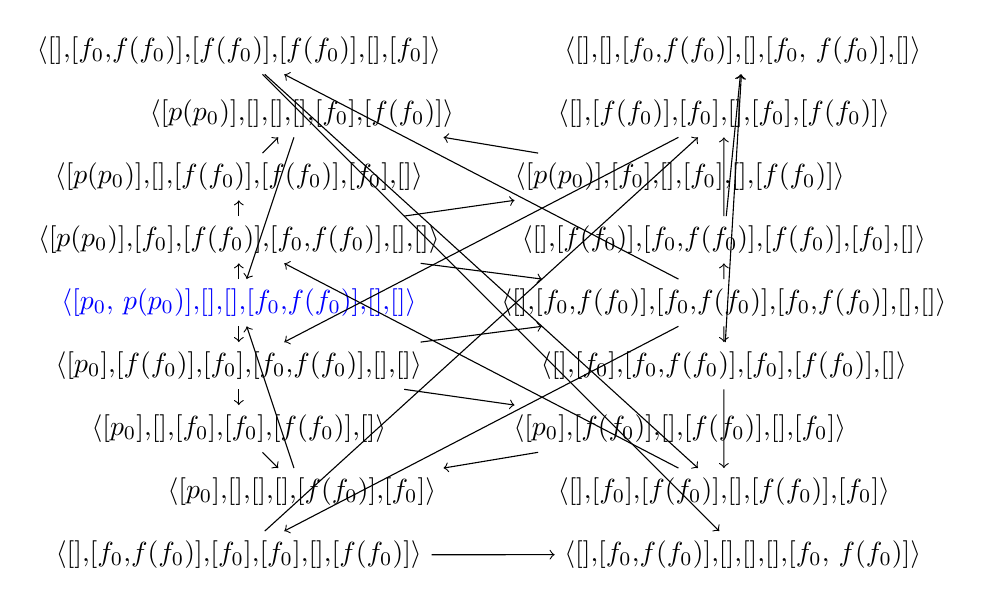
\begin{tikzpicture}[scale=0.8]
\node[blue] (p1) at (0,0) {$\langle$[$p_0$, $p(p_0)$],[],[],[$f_0$,$f(f_0)$],[],[]$\rangle$};

\node (p11) at (0, 1) {$\langle$[$p(p_0)$],[$f_0$],[$f(f_0)$],[$f_0$,$f(f_0)$],[],[]$\rangle$};

\node (p12) at (0, -1) {$\langle$[$p_0$],[$f(f_0)$],[$f_0$],[$f_0$,$f(f_0)$],[],[]$\rangle$};

\node (p111) at (0, 2) {$\langle$[$p(p_0)$],[],[$f(f_0)$],[$f(f_0)$],[$f_0$],[]$\rangle$};

\node (p112) at (7, 2) {$\langle$[$p(p_0)$],[$f_0$],[],[$f_0$],[],[$f(f_0)$]$\rangle$};

\node (p11e) at (1, 3) {$\langle$[$p(p_0)$],[],[],[],[$f_0$],[$f(f_0)$]$\rangle$};

\node (p121) at (0, -2) {$\langle$[$p_0$],[],[$f_0$],[$f_0$],[$f(f_0)$],[]$\rangle$};

\node (p122) at (7, -2) {$\langle$[$p_0$],[$f(f_0)$],[],[$f(f_0)$],[],[$f_0$]$\rangle$};

\node (p12e) at (1, -3) {$\langle$[$p_0$],[],[],[],[$f(f_0)$],[$f_0$]$\rangle$};

\node (p2) at (7.7, 0) {$\langle$[],[$f_0$,$f(f_0)$],[$f_0$,$f(f_0)$],[$f_0$,$f(f_0)$],[],[]$\rangle$};

\node (p21) at (7.7, 1) {$\langle$[],[$f(f_0)$],[$f_0$,$f(f_0)$],[$f(f_0)$],[$f_0$],[]$\rangle$};

\node (p22) at (7.7, -1) {$\langle$[],[$f_0$],[$f_0$,$f(f_0)$],[$f_0$],[$f(f_0)$],[]$\rangle$};

\node (p211) at (7.7, 3) {$\langle$[],[$f(f_0)$],[$f_0$],[],[$f_0$],[$f(f_0)$]$\rangle$};

\node (p221) at (7.7, -3) {$\langle$[],[$f_0$],[$f(f_0)$],[],[$f(f_0)$],[$f_0$]$\rangle$};

\node (p2111) at (8, 4) {$\langle$[],[],[$f_0$,$f(f_0)$],[],[$f_0$, $f(f_0)$],[]$\rangle$};

\node (p23) at (0, 4) {$\langle$[],[$f_0$,$f(f_0)$],[$f(f_0)$],[$f(f_0)$],[],[$f_0$]$\rangle$};

\node (p24) at (0, -4) {$\langle$[],[$f_0$,$f(f_0)$],[$f_0$],[$f_0$],[],[$f(f_0)$]$\rangle$};

\node (p2112) at (8, -4) {$\langle$[],[$f_0$,$f(f_0)$],[],[],[],[$f_0$, $f(f_0)$]$\rangle$};

\begin{scope}[every path/.style={->}]
       \draw (p1) -- (p11);
       \draw (p1) -- (p12); 
       \draw (p11) -- (p111); 
       \draw (p11) -- (p112); 
       \draw (p111) -- (p11e); 
       \draw (p112) -- (p11e); 
       \draw (p11e) -- (p1); 
       \draw (p12) -- (p121); 
       \draw (p12) -- (p122); 
       \draw (p121) -- (p12e);
       \draw (p122) -- (p12e);
       \draw (p12e) -- (p1);
       \draw (p11) -- (p2);
       \draw (p12) -- (p2);
		\draw (p2) -- (p21);
		\draw (p2) -- (p22);       
		\draw (p21) -- (p211);
		\draw (p22) -- (p221);
       \draw (p211) -- (p12);
       \draw (p221) -- (p11);
       \draw (p21) -- (p2111);
       \draw (p22) -- (p2111);
   		\draw (p2) -- (p23);
		\draw (p2) -- (p24);       
		\draw (p23) -- (p221);       
		\draw (p24) -- (p211);       
		\draw (p23) -- (p2112);       
		\draw (p24) -- (p2112);       
\end{scope} 

\end{tikzpicture}

\end{center}
\end{frame}



\begin{frame}{Verificarea modelelor - AlPiNA - Prânzul filosofilor}
\begin{figure}
\centering
\includegraphics[scale=0.32]{images/alpina7}
\end{figure}
\end{frame}



\begin{frame}{Verificarea modelelor - AlPiNA - Prânzul filosofilor}
\begin{figure}
\centering
\includegraphics[scale=0.32]{images/alpina8}
\end{figure}
\end{frame}



\begin{frame}{Verificarea modelelor - AlPiNA - Prânzul filosofilor}
\begin{center}

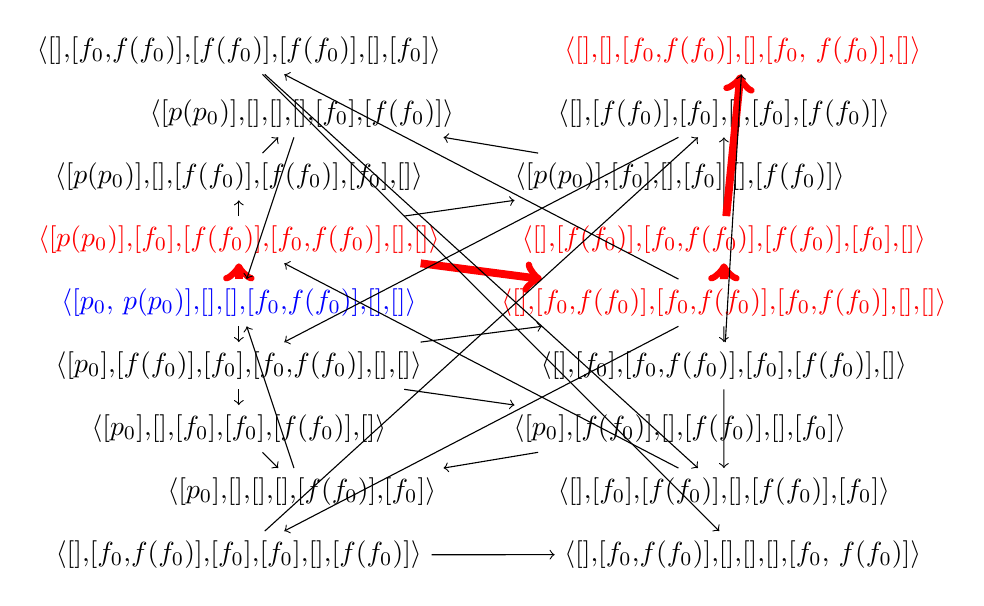
\begin{tikzpicture}[scale=0.8]
\node[blue] (p1) at (0,0) {$\langle$[$p_0$, $p(p_0)$],[],[],[$f_0$,$f(f_0)$],[],[]$\rangle$};

\node[red] (p11) at (0, 1) {$\langle$[$p(p_0)$],[$f_0$],[$f(f_0)$],[$f_0$,$f(f_0)$],[],[]$\rangle$};

\node (p12) at (0, -1) {$\langle$[$p_0$],[$f(f_0)$],[$f_0$],[$f_0$,$f(f_0)$],[],[]$\rangle$};

\node (p111) at (0, 2) {$\langle$[$p(p_0)$],[],[$f(f_0)$],[$f(f_0)$],[$f_0$],[]$\rangle$};

\node (p112) at (7, 2) {$\langle$[$p(p_0)$],[$f_0$],[],[$f_0$],[],[$f(f_0)$]$\rangle$};

\node (p11e) at (1, 3) {$\langle$[$p(p_0)$],[],[],[],[$f_0$],[$f(f_0)$]$\rangle$};

\node (p121) at (0, -2) {$\langle$[$p_0$],[],[$f_0$],[$f_0$],[$f(f_0)$],[]$\rangle$};

\node (p122) at (7, -2) {$\langle$[$p_0$],[$f(f_0)$],[],[$f(f_0)$],[],[$f_0$]$\rangle$};

\node (p12e) at (1, -3) {$\langle$[$p_0$],[],[],[],[$f(f_0)$],[$f_0$]$\rangle$};

\node[red] (p2) at (7.7, 0) {$\langle$[],[$f_0$,$f(f_0)$],[$f_0$,$f(f_0)$],[$f_0$,$f(f_0)$],[],[]$\rangle$};

\node[red] (p21) at (7.7, 1) {$\langle$[],[$f(f_0)$],[$f_0$,$f(f_0)$],[$f(f_0)$],[$f_0$],[]$\rangle$};

\node (p22) at (7.7, -1) {$\langle$[],[$f_0$],[$f_0$,$f(f_0)$],[$f_0$],[$f(f_0)$],[]$\rangle$};

\node (p211) at (7.7, 3) {$\langle$[],[$f(f_0)$],[$f_0$],[],[$f_0$],[$f(f_0)$]$\rangle$};

\node (p221) at (7.7, -3) {$\langle$[],[$f_0$],[$f(f_0)$],[],[$f(f_0)$],[$f_0$]$\rangle$};

\node[red] (p2111) at (8, 4) {$\langle$[],[],[$f_0$,$f(f_0)$],[],[$f_0$, $f(f_0)$],[]$\rangle$};

\node (p23) at (0, 4) {$\langle$[],[$f_0$,$f(f_0)$],[$f(f_0)$],[$f(f_0)$],[],[$f_0$]$\rangle$};

\node (p24) at (0, -4) {$\langle$[],[$f_0$,$f(f_0)$],[$f_0$],[$f_0$],[],[$f(f_0)$]$\rangle$};

\node (p2112) at (8, -4) {$\langle$[],[$f_0$,$f(f_0)$],[],[],[],[$f_0$, $f(f_0)$]$\rangle$};

\begin{scope}[every path/.style={->}]
       \draw[line width=1mm, red] (p1) -- (p11);
       \draw (p1) -- (p12); 
       \draw (p11) -- (p111); 
       \draw (p11) -- (p112); 
       \draw (p111) -- (p11e); 
       \draw (p112) -- (p11e); 
       \draw (p11e) -- (p1); 
       \draw (p12) -- (p121); 
       \draw (p12) -- (p122); 
       \draw (p121) -- (p12e);
       \draw (p122) -- (p12e);
       \draw (p12e) -- (p1);
       \draw[line width=1mm, red] (p11) -- (p2);
       \draw (p12) -- (p2);
		\draw[line width=1mm, red] (p2) -- (p21);
		\draw (p2) -- (p22);       
		\draw (p21) -- (p211);
		\draw (p22) -- (p221);
       \draw (p211) -- (p12);
       \draw (p221) -- (p11);
       \draw[line width=1mm, red] (p21) -- (p2111);
       \draw (p22) -- (p2111);
   		\draw (p2) -- (p23);
		\draw (p2) -- (p24);       
		\draw (p23) -- (p221);       
		\draw (p24) -- (p211);       
		\draw (p23) -- (p2112);       
		\draw (p24) -- (p2112);       
\end{scope} 

\end{tikzpicture}

\end{center}
\end{frame}



\begin{frame}{Verificarea modelelor - AlPiNA - Prânzul filosofilor}
Exerciţii:

\begin{itemize}
\item
Doi filosofi vecini pot mânca în acelaşi timp?

\textbf{!exists(\$f1 in HasL, \$f2 in HasR : \$f1 = \$f2);}

\item
Doi filosofi aflaţi faţă în faţă pot mânca în acelaşi timp?

...
\item
Se poate întâmpla ca filosofii să flămânzească până la moarte?

\textbf{Deadlock;}

\item
Un anume filosof poate mânca în cele din urmă (presupunând că doreşte să facă acest lucru)?

\textbf{forall(\$x in Think : \$x != p0) \& exists(\$f1 in HasL : \$f1 = f0) \& exists(\$f2 in HasR : \$f2 = f(f0));}

\end{itemize}
\end{frame}


\begin{frame}{Verificarea modelelor - AlPiNA - Prânzul filosofilor}

\begin{table}[h]
\centering
\begin{tabular}{c r r r}
\hline
Number of philosophers & Number of states\\
\hline
2       &      18\\ %&         1.67 &       982\\ % cache hits to rewrites ratio: 72%
3       &      76\\ %&         3.27 &     1253\\ % cache hits to rewrites ratio: 78%
4       &     322\\ %&       10.04 &     4883\\ % cache hits to rewrites ratio: 83%
5       &    1364\\ %&       51.74 &   12334\\ % cache hits to rewrites ratio: 86%
6       &    5778\\ %&     327.60 &   38802\\ % cache hits to rewrites ratio: 88%
7       &   24476\\ %&   2676.35 &   98751\\ % cache hits to rewrites ratio: 22%
8       &  103682\\ %& 27592.29 & 152628\\ % cache hits to rewrites ratio: 4%
$\dots$ & $\dots$\\
200     & $2.5 \times 10^{125}$\\
\hline
\end{tabular}
\caption{Evoluţia dimensiunii spaţiului stărilor în funcţie de numărul de filosofi}
\label{table:quantdata6}
\end{table}
\end{frame}



\begin{frame}{Problema exploziei spaţiului stărilor}
Explozia spaţiului stărilor constă în existenţa unui număr foarte mare de stări în care sistemul poate să ajungă, chiar şi pentru modele de dimensiuni mici

\vspace{0.5cm}

Cauzele exploziei spaţiului stărilor pot fi:
\begin{itemize}
\item
concurenţa
\item
variabilele care pot lua o gamă largă de valori (în cazul lmbajelor de modelare care permit utilizarea variabilelor)
\item
numărul mare de variabile de care depinde modelul
\end{itemize}
\end{frame}



\begin{frame}{Contramăsuri la problema exploziei spaţiului stărilor}
\begin{itemize}
\item
\textbf{Abstractizarea} - eliminarea informaţiilor irelevante şi simplificarea modelului
\item
\textbf{Compresia} - operaţiile se fac asupra unor \textbf{mulţimi de stări}, pentru codarea cărora se folosesc structuri eficiente (BDD: Binary Decision Diagrams) - Symbolic Model Checking
\item
\textbf{Reducerea} - evitarea explorării multiple a execuţiilor echivalente, reducându-se astfel numărul de combinaţii considerate

ex: dacă pentru verificarea în curs nu contează care dintre procesele P şi Q se execută primul, nu este nevoie să fie analizată şi varianta PQ, şi varianta QP, fiind suficientă analiza uneia dintre ele
\end{itemize}
\end{frame}



\begin{frame}{Perspective multiple asupra aceluiaşi sistem}
Există multiple pentru descrierea sistemelor:
\begin{itemize}
\item
reţele Petri (foarte multe tipuri)
\item
unele limbaje de programare (ex: PROMELA)
\item
communicating automata
\item
process algebra
\item
limbaje descriptive semi-formale (ex: UML)
\end{itemize}

\vspace{0.5cm}

Alegerea se face în funcţie de:
\begin{itemize}
\item
tipul sistemului modelat
\item
tipul proprietăţilor care vor fi verificate
\item
precizia urmărită
\end{itemize}
\end{frame}



\begin{frame}{Verificarea modelelor}
Verificatoare de modele:
\begin{itemize}
\item
exemplele anterioare pentru reţele Petri
\newline

\item
\textbf{FDR4} - CSP (Communicating Sequential Processes)

\url{https://www.cs.ox.ac.uk/projects/fdr/}
\newline

\item
\textbf{LTSmin} - language independent (process algebra, timed automata, DiVinE, PROMELA, etc.)

\url{http://fmt.cs.utwente.nl/tools/ltsmin/}
\newline
\end{itemize}
\end{frame}



\begin{frame}{Verificarea modelelor}
Verificatoare de modele:
\begin{itemize}
\item
\textbf{SPIN} - PROMELA

\url{http://spinroot.com/spin/whatispin.html}
\newline

\item
\textbf{UPPAAL} - networks of timed automata extended with data types

\url{http://www.uppaal.org/}
\newline

\item
\textbf{StrataGEM} - 

\url{https://github.com/mundacho/stratagem}
\newline
\item
etc.
\end{itemize}
\end{frame}



\begin{frame}{Demonstrarea teoremelor}
Verificarea valorii de adevăr a teoremelor matematice postulate despre un sistem. 

\vspace{0.5cm}

Etape:
\begin{enumerate}
\item
Stabilirea axiomelor
\item
Stabilirea concluziilor
\item
Demonstraţia propriu-zisă

- foloseşte regulile inferenţei logice pentru a stabili dacă concluziile sunt adevărate sau false
\end{enumerate}

\vspace{0.5cm}

Constă mai mult dintr-un proces interactiv: necesită \textbf{intervenţia utilizatorului} pentru a ghida instrumentul în direcţia corectă

\vspace{0.5cm}

\textbf{Mult mai puţin automatizabilă decât metoda verificării modelelor}
\end{frame}



\begin{frame}[fragile]{Demonstrarea teoremelor - Un exemplu foarte simplu}
\begin{verbatim}
theorem and_commutative (p q : Prop) : p ∧ q → q ∧ p :=
assume Hpq : p ∧ q,
have Hp : p, from and.elim_left Hpq,
have Hq : q, from and.elim_right Hpq,
show q ∧ p, from and.intro Hq Hp
\end{verbatim}

Din "Theorem proving in Lean" - \url{https://leanprover.github.io/tutorial/}
\end{frame}



\begin{frame}{Demonstrarea teoremelor}
Demonstratoare automate de teoreme:

\begin{itemize}
\item
\textbf{ACL2} - \url{http://www.cs.utexas.edu/users/moore/acl2/}: high order logic
\item
\textbf{Coq} - \url{https://coq.inria.fr/}: high order logic
\item
\textbf{E} - \url{http://wwwlehre.dhbw-stuttgart.de/~sschulz/E/E.html}: first order logic
\item
\textbf{HOL} - \url{http://www.cl.cam.ac.uk/research/hvg/HOL/}: high order logic
\item
\textbf{Prover9} - \url{http://www.cs.unm.edu/~mccune/prover9/}: 1st order logic
\item
etc.
\end{itemize}
\end{frame}



\begin{frame}{Verificarea echivalenţei}
Procesul verificării dacă două \textbf{implementări ale aceluiaşi sistem}, la nivele diferite de abstractizare, \textbf{sunt identice}

\vspace{0.5cm}

\begin{itemize}
\item
Nu poate fi folosită pentru a verifica dacă un sistem are sau nu erori
\item
Ci numai pentru a semnala dacă între două implementări există sau nu diferenţe funcţionale
\end{itemize}

\vspace{0.5cm}

Se utilizează pe larg în industrie

ex: proiectarea circuitelor integrate digitale

\end{frame}



\begin{frame}{Verificarea echivalenţei}
Verificatoare de echivalenţă:

\begin{itemize}
\item
\textbf{CADP} - acceptă o gamă largă de formalisme de intrare

\url{http://cadp.inria.fr/}
\newline

\item
\textbf{SYNOPSYS} - circuite hardware

\url{http://www.synopsys.com/Tools/Verification/FormalEquivalence/Pages/default.aspx}
\newline

\item
\textbf{Xilinx} - FPGA

\url{http://www.xilinx.com/}
\newline

\item
etc.
\end{itemize}

\end{frame}



\begin{frame}{Verificarea formală a protocoalelor de securitate}
\begin{enumerate}
\item
Modelarea a componentelor sistemului
\begin{enumerate}
\item
reţeaua
\item
adversarul
\item
protocolul de securitate
\end{enumerate}
\item
Specificarea proprietăţilor de securitate care trebuie verificate
\begin{itemize}
\item
autentificarea
\item
confidenţialitatea
\item
integritatea
\item
non-repudierea
\item
disponibilitatea
\end{itemize}
\item
Verificarea propriu-zisă
\end{enumerate}
\end{frame}



\begin{frame}{Modelul reţelei}

Este furnizat de către instrumentul de verificare formală

\vspace{0.5cm}

Reţeaua - colecţia tuturor \textbf{nodurilor oneste, plus adversarul}

Nodurile:
\begin{itemize}
\item
statice
\item
identificate printr-un nume unic
\item
o singură interfaţă de comunicaţie
\item
adversarul are mai mult de o interfaţă - este modelat sub forma mai multor noduri
\item
legături simetrice: dacă un nod oarecare A poate să primească o transmisie de la un nod B, atunci şi nodul B poate să primească o transmisie de la nodul A
\end{itemize}

\end{frame}



\begin{frame}{Modelul adversarului}

Este furnizat de către instrumentul de verificare formală

\vspace{0.5cm}

Adversar - nod care are ca şi scop \textbf{devierea} şi \textbf{alterarea în mod activ} a rulării protocolului de securitate

\vspace{0.5cm}

Acţiunile adversarului depind de protocolul de securitate ţintă

\vspace{0.5cm}

Adversarul \textbf{apare ca fiind un utilizator legitim} al reţelei, putând iniţia o conversaţie cu orice alt nod din reţea

\end{frame}



\begin{frame}{Modelul adversarului - Capabilităţi}
\textbf{Modelul Dolev-Yao} (modelul adversarului puternic) 

\vspace{0.5cm}

Adversarul poate:
\begin{itemize}
\item
genera orice tip de mesaj din protocolul ţintă
\item
intercepta mesajele oricărui nod din reţea
\item
răspunde la orice tip de mesaj primit/interceptat
\item
cripta/decripta mesaje folosind cheile pe care le cunoaşte
\item
modifica orice mesaj primit/interceptat
\end{itemize}

\vspace{0.5cm}

\textbf{Adversarul este reţeaua, şi reţeaua este adversarul}

\end{frame}



\begin{frame}{Modelul adversarului - restricţii}
Singura restricţie - puterea finită de calcul

\begin{itemize}
\item
Nu este în măsură să lanseze atacuri cripto analitice cu scopul de a compromite chei simetrice sau asimetrice
\item
Nu poate inversa funcţiile folosite pentru hash
\end{itemize}

\end{frame}



\begin{frame}{Modelul protocolului de securitate}
Trebuie realizat de către persoana care face verificarea

\vspace{0.5cm}

Depinde de limbajul de modelare acceptat de către instrumentul de verificare formală

\vspace{0.5cm}

Utilizatorul specifică apoi proprietăţile de securitate pe care doreşte să le verifice

\end{frame}



\begin{frame}{Verificarea propriu-zisă}
Depinde de instrumentul de verificare formală utilizat

\vspace{0.5cm}

Intrări:
\begin{itemize}
\item
modelul protocolului de securitate
\item
proprietăţile de securitate care trebuie verificate
\end{itemize}

Ieşire:
\begin{itemize}
\item
proprietăţile de securitate sunt îndeplinite
\item
proprietăţile de securitate NU sunt îndeplinite
\begin{itemize}
\item
contraexemplu - \textbf{un exemplu de atac}
\end{itemize}
\end{itemize}
\end{frame}



\begin{frame}{Verificarea formală a protocoalelor de securitate}
Verificatoare de modele specializate pe probleme de securitate:
\begin{itemize}
\item
\textbf{AVISPA}

\url{http://www.avispa-project.org/}
\newline

\item
\textbf{AVANTSSAR}

\url{http://www.avantssar.eu/}
\newline

\item
\textbf{Casper \& FDR2}

\url{http://www.cs.ox.ac.uk/gavin.lowe/Security/Casper/}

(latest version \textbf{FDR4} - \url{https://www.cs.ox.ac.uk/projects/fdr/})
\newline

\end{itemize}
\end{frame}



\begin{frame}{Verificarea formală a protocoalelor de securitate}
Verificatoare de modele specializate pe probleme de securitate:
\begin{itemize}
\item
\textbf{SPaCIoS} 

\url{http://www.spacios.eu/}
\newline

\item
\textbf{ProVerif}

\url{http://prosecco.gforge.inria.fr/personal/bblanche/proverif/}
\newline

\item
\textbf{Scyther}

\url{https://www.cs.ox.ac.uk/people/cas.cremers/scyther/}
\newline

\item
etc.
\end{itemize}
\end{frame}



\begin{frame}{Bibliografie}
\begin{itemize}
\item
John Franco, \textbf{Formal Methods}, University of Cincinnati

\url{http://gauss.ececs.uc.edu/Courses/c626/lectures.html}
\newline

\item
Vasileios Koutavas, \textbf{Formal Verification}, University of Dublin

\url{https://www.scss.tcd.ie/Vasileios.Koutavas/teaching/cs4004-4504/mt1819/}
\newline

\item
Radek Pelanek, \textbf{Formal Verification and Model Checking}, Masaryk University

\url{https://www.fi.muni.cz/~xpelanek/IA158/slides/verification.pdf}
\end{itemize}
\end{frame}



\end{document}